\documentclass[journal, twocolumn]{IEEEtran}
%\usepackage[switch]{lineno}
\usepackage[utf8]{inputenc}
\usepackage{graphicx}
\usepackage{amsmath}
\usepackage{float}
\usepackage{caption}
\usepackage{url}
\usepackage{pdfpages}
\usepackage{setspace}
\usepackage{multicol}
\usepackage{multirow}
\usepackage{tabularx}
\usepackage{booktabs}
\usepackage[colorlinks, citecolor=blue]{hyperref}
\usepackage[numbers, sort]{natbib}
\usepackage{others/aastex_hack}
\usepackage{subfloat}
\usepackage{siunitx}
\usepackage{xcolor}
\usepackage{subfiles}

\usepackage{longtable}

\newcolumntype{C}{>{\centering\arraybackslash}X} % centered version of "X" type
\setlength{\extrarowheight}{1pt}
\DeclareSIUnit{\parsec}{pc}
\DeclareSIUnit{\yr}{yr}
\DeclareSIUnit{\Msun}{M_\odot}

\newcommand{\kpc}{\kilo\parsec}
\newcommand{\lowalpha}{low-$[\alpha/\text{Fe}]$}
\newcommand{\highalpha}{high-$[\alpha/\text{Fe}]$}
\newcommand{\feh}{[\text{Fe}/\text{H}]}
\newcommand{\mone}[1]{m_{1_{\text{#1}}}}
\newcommand{\mtwo}[1]{m_{2_{\text{#1}}}}
\newcommand{\semaxis}[1]{a_{\text{#1}}}
\newcommand{\ecc}[1]{e_\text{#1}}
\newcommand{\interval}[1]{t_\text{#1}}

\if
CLASSINFOpdf
\else
\fi

\title{Detecting gravitational waves sources $-$ BHBH, NSNS, BHNS $-$ with LISA}
\author{
    \IEEEauthorblockN{Nazeela Aimen},
    \IEEEauthorblockN{Syed Ali Mohsin Bukhari},
    \IEEEauthorblockN{Asad Ali}
    \and\\
    \IEEEauthorblockA{
        \textit{
            Department of Applied Mathematics and Statistics, Institute of Space Technology, Islamabad 44000, Pakistan.
        }\\
    }
    \IEEEauthorblockA{
        \textit{
            Space and Astrophysics Research Lab (SARL), Institute of Space Technology, Islamabad 44000, Pakistan.
        }
    }
}

\markboth{Journal of- \LaTeX\ Class Files,~Vol.~14, No.~8, August~2015}%
{Shell \MakeLowercase{\textit{et al.}}: Bare Demo of IEEEtran.cls for IEEE Journals}

\begin{document}
%    \bstctlcite{IEEEexample:BSTcontrol}
    \maketitle
    \IEEEpeerreviewmaketitle
    \begin{abstract}
        \, \color{red}{Abstract is still missing!!}
    \end{abstract}
    \begin{IEEEkeywords}
        Cobb-Douglas Habitability Score, Exoplanets, Habitability, Habitable zone, Convex Optimization, Duality.
    \end{IEEEkeywords}

%    \linenumbers


    \section{Introduction}
    \label{sec:intro}
    The gravitational waves (GW) were predicted a year after the final formulation of the general theory of relativity (GR) by Albert Einstein~\cite{Einstein1916}.
    Similar to electromagnetic waves, the GWs travel at the speed of light~\citep{Eddington1922, Abott2017}.
    However, unlike electromagnetic waves, the GW stretches and squeezes the space itself thus causing spatial disturbances.
    The detection of Hulse-Taylor binary~\citep{Hulse1975}, and the subsequent observation of a seven years time
    span~\citep{Taylor1982} stirred a great interest in the GW observations.
    It wasn't until 2015 that the first direct observation of GW was made by LIGO and VIRGO collaborations~\citep{Abott2017}.
    The lower frequency bound for both the aLIGO and VIRGO detectors is around \SI{10}{\hertz}~\cite{aLIGO2015, aVIRGO2014}

    The Laser Interferometer Space Antenna (LISA) has three spacecrafts that form a triangle, each side 2.5 million
    km long~\cite{Prince2002, Robson2019}.
    Operating in the frequency range of \SI{1e-5}{\hertz}$\,\leq  f \leq\,$\SI{1e-1}{\hertz} LISA will be able to observe the sources millions of years before they merge.
    The early detection capability will help better constrain and determine the orbital parameters of the observed binaries.
    Some sources detectable by LISA are the extreme mass ratio inspirals (EMRIs)~\cite{Gair2017, Klein2016, Chapman2022} and galactic binaries~\cite{wagg2021gravitational, Abott2017, Digman2022}.
    This makes LISA also capable of mapping Milky Way galaxy's structure.
    Another interesting class detectable by LISA is the double white dwarf stars (DWDs) which are reported to be abundant in our MW galaxy and have a substantial detection in LISA as well~\cite{Korol2017, Nelemans2001, Willems2007, Ruiter2010}.

    A lot of effort has been put into the detection of potential GW sources for LISA, the resolution of issues that might be associated with the background data, and proposals of new candidates as GW sources for LISA~\cite[see, for example,][]{Lau2020, Sesana2009, Khakhaleva2020, Renzo2021, Fumagalli2022, wagg2021gravitational, Broekgaarden2021, Shao2021, Andrews2020, Belczynski2010, Guo2017, Babak2010, Blaut2010, Babak2008, Ruiter2010, Nelemans2001, Yu2010}.
    The detections of these sources will provide us with a better understanding of not only the evolution phases but also the endpoints of stellar evolution.

    The goals of this research are,
    \begin{itemize}%
        \item to predict the number of DCO binaries that can be detected via LISA in our Milky Way galaxy,
        \item to determine whether extra galactic sources are LISA detectable,
        \item to make a general detection comparison between DCO binaries with and without an initial eccentricity.
    \end{itemize}%

    This research paper is structured as follows, in section~\ref{sec:population_synthesis} we discuss the generation of binary systems using COMPAS suite.
    In section~\ref{sec:evolution-methodology} we give a general overview of the methodology adopted in this research for evolving the stars from ZAMS to DCOs, from DCOs to merger stage, and their detection by LISA as well.
    The evolution of binaries and their detection is discussed in section~\ref{sec:evolution-and-detection}.


    \section{Population synthesis}
    \label{sec:population_synthesis}
    The population synthesis for the detections of the double compact objects (DCOs) was performed using the Compact Object Mergers: Population Astrophysics and Statistics (COMPAS; ~\cite{stevenson2017formation, Riley2022, Vigna2018}) suite.
    COMPAS is a rapid stellar evolution suite and can evolve both single and binary stars following the details outlined by~\cite{Hurley2000, Hurley2002}.
    A list of selected papers that make use of the COMPAS suite is also available on the COMPAS website.\footnote{\url{https://compas.science/science.html}}

    This study makes use exclusively of the binary star evolution (BSE) synthesis method.
    The default parameters used by the COMPAS software are listed in table 1 in the COMPAS paper~\cite{Riley2022}.

    Except for supernova mass remnant prescription, initial eccentricity ($e_i$), metallicity ($z$), and pulsar evolution, all other parameters were taken at the default value.
    For a one-to-one correspondence between the two generated data sets, the seed numbers were kept constant.

    For the mass of primary star, we draw the values from Kroupa initial mass function (IMF) with $m_1 \in [5, 150]\,\text{M}_\sun$~\cite{kroupa2001variation}.
    For the secondary star, we randomly draw from uniform distribution to satisfy $q\equiv m_2/m_1$, where $q\,\in\,[0, 1]$~\cite{sana2012binary}.
    An additional constraint of $m_2 \geq 0.1\,m_1$ was placed on $m_2$ as this is the minimum mass necessary for a star to be considered as a main sequence star.

    For the semi-major axis of the binary, we drew the parameter values from a flat-in-the-log distribution with $a_i \in [0.1, 1000]\,$AU, such that $p(a_i) \propto 1/a_i$~\cite{opik1924photographic}.

    For the remnant mass prescription, we first considered the Fryer delayed model~\cite{Fryer2012}.
    However, this resulted in a concentration of NS mass around $\sim1.28\,\text{M}_\odot$.
    To avoid this concentration of NS final mass, we used Müller \& Mandel prescription (M\&M)~\cite{Mandel2020}.
    M\&M is a stochastic remnant mass model that offers a smoother mass distribution for NS\@.
    We also switched the \textbf{evolve\_pulsar} flag to \textbf{True} during population synthesis.

    For metallicity, we drew the values from a $\text{Beta}(5, 80)$ distribution.
    The main motivation behind the selection of such biased distribution is the higher metallic content of present-day stars.
    The population III stars were primarily composed of pure hydrogen and their deaths produced heavier metals in the Universe.
    By this extension, the stars that are present now or those that will merge now must have higher metallic content.
    As such, we also speculate that having stars with higher metallic content might produce more NSNS or NS-BH pairs for detection rather than BHBH pairs.

    For eccentricity, we make use of two cases,
    \begin{itemize}
        \item Case I: All the binary systems are generated using a flat distribution, $e \in (0, 1)$.
        \item Case II: All the binary systems are generated with circular orbits, i.e., $e = 0$.
    \end{itemize}

    Details about the selection of metallicity and eccentricity values in COMPAS are provided in appendix~\ref{sec:appA}.
%    In section~\ref{sec:detections} we discuss the summary of the DCOs formed by the COMPAS generated binaries.
%    In addition to the parameter mentioned above, the COMPAS chooses four more parameters stochastically.
%    Including kick random magnitude, kick phi, kick theta, and kick mean anomaly.


    \section{Evolution methodology}
    \label{sec:evolution-methodology}
    We first generated \num{1e7} values for metallicity using the beta distribution within the COMPAS limits.
%    The values were stored in ten separate grid files and used with COMPAS to simulate the binaries.
    We denote the zero-age main sequence (ZAMS) parameters of the binaries as,
    \begin{equation}%
        \mone{ZAMS}, \mtwo{ZAMS}, \semaxis{ZAMS}, \ecc{ZAMS}, Z, \o
        \label{eq:zams_parameter_names}
    \end{equation}%
    COMPAS evolves the binaries up to \SI{13.7}{\giga\yr}.
    We represent the resulting double compact object (DCO) parameters as,
    \begin{equation}%
        \mone{DCO}, \mtwo{DCO}, \semaxis{DCO}, \ecc{DCO}, \interval{evolve}, Z, \o,
        \label{eq:dco_parameter_names}
    \end{equation}%
    where $Z$ is the metallicity of the binary system, $\o$ is the seed number, $\interval{evolve}$ is the time required to form DCO from ZAMS. $\semaxis{ZAMS}$, $\semaxis{DCO}$, $\ecc{ZAMS}$, and $\ecc{DCO}$ are the semi-major axis and eccentricity of the binary orbit at ZAMS and DCO formation respectively.
    \begin{figure}[!ht]%
        \centering%
        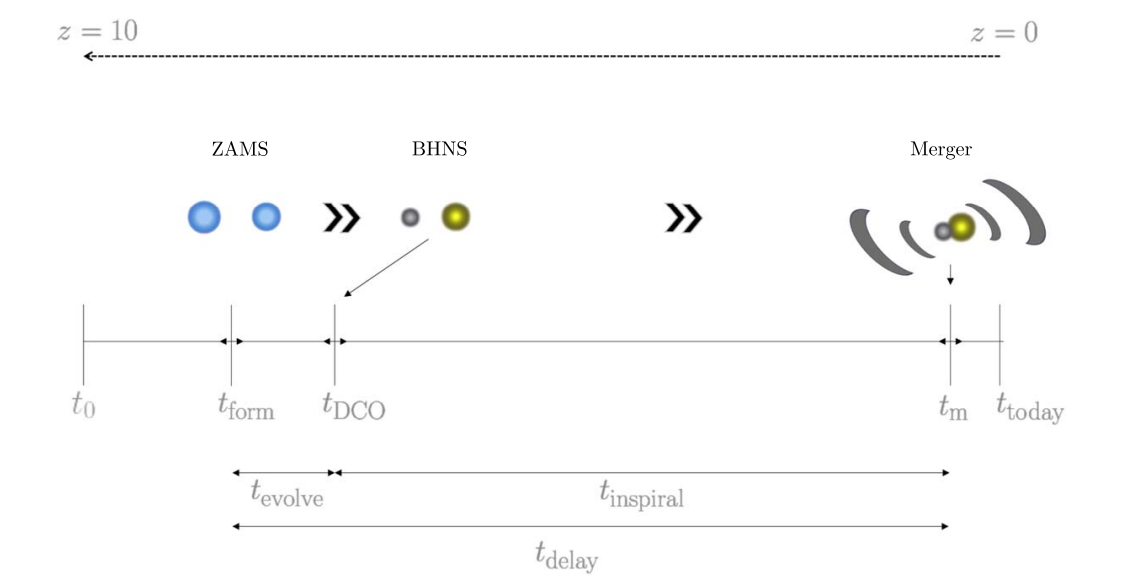
\includegraphics[width=\linewidth]{images/binary_evolution}%
        \caption{Schematic diagram showing various time intervals for a binary system from ZAMS formation, to DCO, and merger. The figure is taken from~\cite{Riley2022}.}%
        \label{fig:binaryevolution}%
    \end{figure}%
    Once the DCOs have been formed, we move out of the COMPAS suite.
    For the LISA detection, the DCO formed from the set of binaries were checked for an evolutionary stop, i.e., only those binaries were selected that will merge within the Hubble time.
    The selected candidates were than provided to the python framework LEGWORK~\cite{wagg2021legwork} that evolved them from the DCO stage to the merger state.
    It evolved the binaries using equations from~\cite{Peters1963, Peters1964}.

    The DCO$-$merger evolution method follows the one outlined by~\cite{wagg2021gravitational} closely.
    The evolution was done such that the MW galaxy instance was divided into bins based on the metallicity values of the evolving binaries.
    The evolution time was calculated after taking into consideration the ZAMS-DCO evolution time and the lookback time of the binary produced.
    If a binary, at DCO stage, had a resultant merger time greater than the difference of its lookback time and ZAMS-DCO evolution time, it was marked as an inspiralling binary.
    Each inspiralling binary was than evolved at every point within the corresponding metallicity bin using LEGWORK to a million year before its merger time.
    At this stage, the resulting LISA parameters of interest were,
    \begin{equation}%
        \semaxis{LISA}, \ecc{LISA}, f_{\text{LISA}}
        \label{eq:lisa_parameter_names}
    \end{equation}%
    The SNR was than calculated by further evolving them for the LISA mission duration of four years.
    The detection is made based on the signal-to-noise ratio (SNR) of the binary averaged over sky position, polarization, and orientation using the following expression from~\cite{Finn2000},
    \begin{equation}
        \rho^2 = \sum_{n=1}^{\infty}\int_{f_{n, i}}^{f_{n, f}}\frac{h_{c, n}^2}{f_n^2 S_n(f_n)}\,\text{d}f_n,
        \label{eq:snr_equation}
    \end{equation}
    where $n$ is the GW harmonic, $f_n$ represents the orbital frequency of $n^\text{th}$ harmonic.
    The parameter $S_n(f_n)$ is the LISA sensitivity curve function~\cite{Robson2019}, and $h_{c, n}$ is the characteristic strain of the $n^\text{th}$ GW harmonic~\cite{Barack2004}.
    \begin{equation}
        h_{c,n}^2 = \frac{2^{5/3}}{3\pi^{4/3}}\frac{(G\mathcal{M}_c)^{5/3}}{c^3 D_L^2}\frac{1}{f_\text{orb}^{1/3}}\frac{g(n, e)}{nF(e)}
        \label{eq:characteristic_strain}
    \end{equation}


    \section{Evolution and detection}
    \label{sec:evolution-and-detection}

    After running the simulations as outlined in section~\ref{sec:population_synthesis}, we obtained 12254 DCOs ($\sim0.12254\%$).
    Following section~\ref{sec:evolution-methodology}, we obtain the required parameter values of only 6539 DCOs that merged within Hubble time ($\sim$53.3622\%) thus making them a potential LISA source.\footnote{Overall, only $\sim$0.06539\% binary system formed into DCOs that merge within Hubble time.}
    The Hubble time merge rate of DCOs is given in table~\ref{tab:dco_details},

    \begin{table}[!ht]
        \centering
%        \resizebox{\columnwidth}{!}{
        \begin{tabular}{@{}cccc@{}}
            \toprule
            \multirow{2.5}{*}{BHBH} & \multirow{2.5}{*}{NSNS} & \multicolumn{2}{c}{BHNS} \\ \cmidrule(l){3-4}
            &           & NSBH    & BHNS     \\ \midrule
            492/663 & 4752/9219 & 480/868 & 815/1504 \\ \bottomrule
        \end{tabular}%
%    	 }
        \caption{Number of DCOs merged within Hubble time vs total DCOs formed by the COMPAS suite.}
        \label{tab:dco_details}
    \end{table}

    The highest merging rate in this study is of BHBH DCO type ($\sim$74.21\%), followed by NSBH pairs ($\sim$55.30\%), BHNS ($\sim$54.2\%) and lastly NSNS DCO type ($\sim$51.55\%) comprising the `candidate binaries'.\footnote{Such DCO pairs which can have a potential LISA detection.}

    \begin{figure*}[!h]%
        \centering
        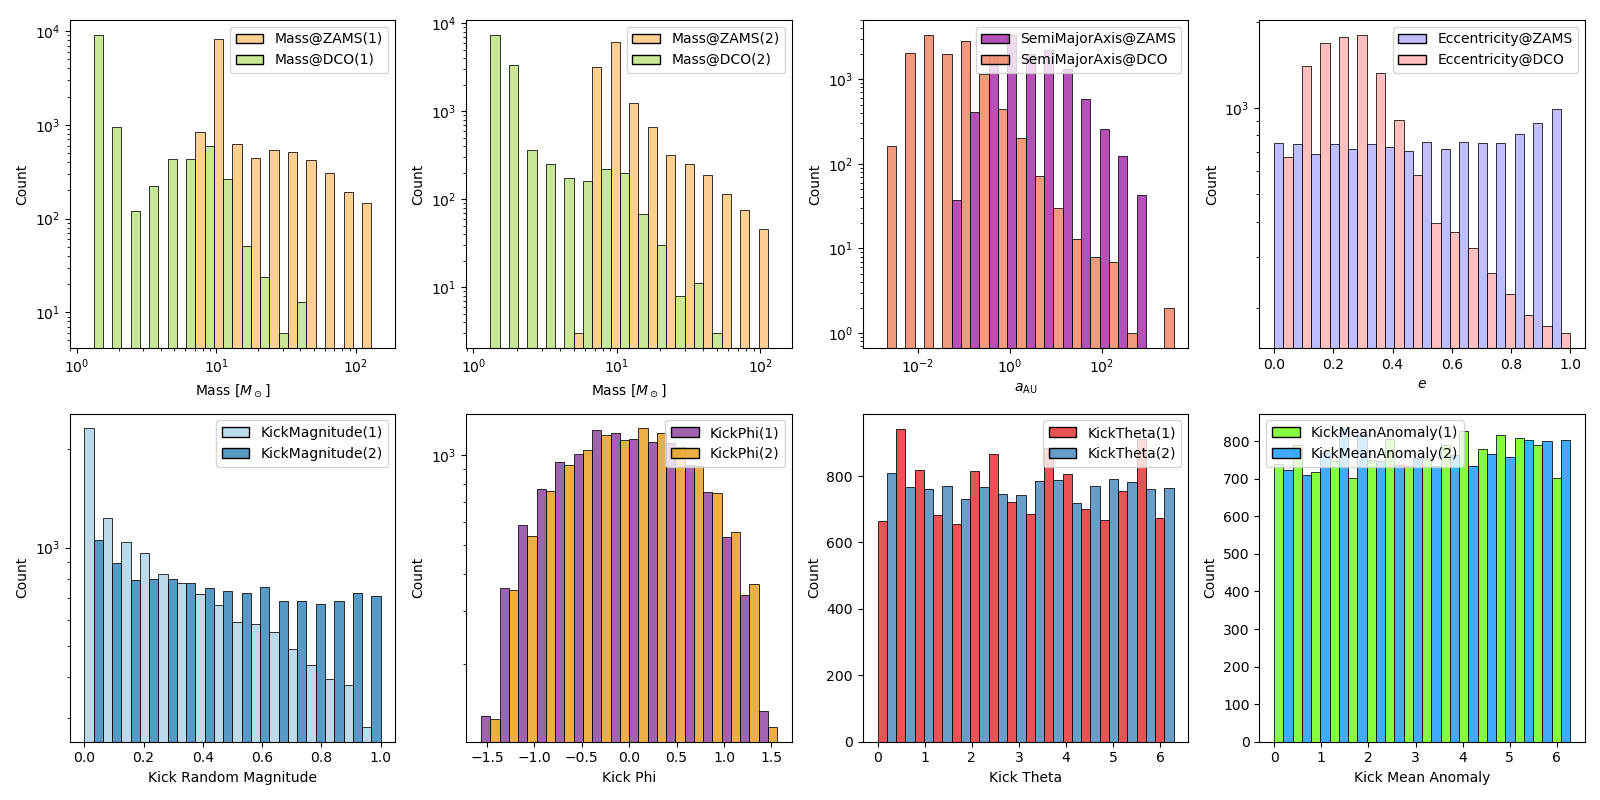
\includegraphics[width=\textwidth]{analysis_data/main_analysis_folder/all_zams_params}
        \caption{The top row shows the distribution of mass, semimajor axis and eccentricity of binary pairs at ZAMS and DCO stage for the `candidate' binaries. The bottom row shows the selection of supernova kick parameters made by the COMPAS suite.}
        \label{fig:all_zams_params}
    \end{figure*}%

    \begin{table*}[!h]
        \centering
        \resizebox{\textwidth}{!}{%
            \begin{tabular}{@{}ccccccccccc@{}}
                \toprule
                \multirow{2.5}{*}{Parameters} & \multirow{2.5}{*}{MAX} & \multicolumn{2}{c}{ZAMS details} & \multicolumn{2}{c}{DCO details} & \multirow{2.5}{*}{MIN} & \multicolumn{2}{c}{ZAMS details} & \multicolumn{2}{c}{DCO details} \\ \cmidrule(lr){3-4} \cmidrule(lr){5-6} \cmidrule(lr){8-9} \cmidrule(lr){10-11}
                &         & Primary & Secondary & Primary & Secondary &        & Primary & Secondary & Primary & Secondary \\ \midrule

                \multicolumn{11}{c}{\textbf{Binary Black Holes}} \\
                $\mone{ZAMS}$ & 149.836 & 149.836 & 115.624   & 10.386  & 10.395    & 13.007 & 13.007  & 12.500    & 2.216   & 2.601     \\
                $\mtwo{ZAMS}$ & 131.178 & 148.802 & 131.178   & 8.662   & 8.459     & 12.500 & 13.007  & 12.500    & 2.216   & 2.601     \\
                $\mone{DCO}$  & 43.308  & 57.334  & 57.334    & 43.308  & 43.308    & 2.022  & 26.497  & 26.493    & 2.022   & 7.104     \\
                $\mtwo{DCO}$  & 43.308  & 57.334  & 57.334    & 43.308  & 43.308    & 2.018  & 42.088  & 30.574    & 7.456   & 2.018     \\

                \multicolumn{11}{c}{\textbf{Binary Neutron Stars}} \\

                $\mone{ZAMS}$ & 54.41   & 54.41   & 13.76     & 1.614   & 1.235     & 8.546  & 8.546   & 7.822     & 1.26    & 1.193     \\
                $\mtwo{ZAMS}$ & 25.571  & 25.586  & 25.571    & 1.480   & 1.693     & 6.626  & 13.01   & 6.626     & 1.26    & 1.194     \\
                $\mone{DCO}$  & 1.938   & 14.022  & 13.938    & 1.938   & 1.487     & 1.135  & 10.319  & 10.019    & 1.135   & 1.392     \\
                $\mtwo{DCO}$  & 1.991   & 13.919  & 13.574    & 1.681   & 1.991     & 1.132  & 11.674  & 11.021    & 1.518   & 1.132     \\

                \multicolumn{11}{c}{\textbf{Neutron Star $-$ Black Hole}} \\

                $\mone{ZAMS}$ & 53.708  & 53.708  & 29.613    & 1.439   & 15.342    & 8.971  & 8.971   & 8.847     & 1.260   & 3.869     \\
                $\mtwo{ZAMS}$ & 42.242  & 42.289  & 42.242    & 1.598   & 7.382     & 8.665  & 9.164   & 8.665     & 1.260   & 2.062     \\
                $\mone{DCO}$  & 1.935   & 14.090  & 13.959    & 1.935   & 3.825     & 1.137  & 27.186  & 17.676    & 1.137   & 9.646     \\
                $\mtwo{DCO}$  & 15.342  & 53.708  & 29.613    & 1.439   & 15.342    & 2.003  & 12.472  & 12.033    & 1.608   & 2.003     \\

                \multicolumn{11}{c}{\textbf{Black Hole $-$ Neutron Star}} \\

                $\mone{ZAMS}$ & 145.467 & 145.467 & 46.439    & 9.907   & 1.593     & 11.626 & 11.626  & 11.608    & 2.216   & 1.522     \\
                $\mtwo{ZAMS}$ & 108.489 & 140.091 & 108.489   & 12.217  & 1.415     & 10.072 & 23.144  & 10.072    & 2.922   & 1.206     \\
                $\mone{DCO}$  & 15.106  & 90.844  & 76.11     & 15.106  & 1.669     & 2.004  & 13.125  & 12.872    & 2.004   & 1.785     \\
                $\mtwo{DCO}$  & 1.945   & 29.142  & 15.445    & 4.341   & 1.945     & 1.141  & 28.317  & 22.834    & 5.61    & 1.141     \\ \bottomrule
            \end{tabular}%
        }
        \caption{Maximum and minimum values for masses of both ZAMS and DCO type stars in the BHBH data set with their respective counterparts. The `MAX' and `MIN' columns represent the maximum and minimum value for the given parameter respectively. The `ZAMS details' and `DCO details' column list the value of primary and secondary components of the binary and `ZAMS' and `DCO' stage of evolution respectively for the binary with `MAX' and `MIN' value of the parameter. All the masses are given in units of solar mass, $M_\odot$ where \num{1}\,$M_\odot \approx$ \SI{2e30}{\kilogram}.}
        \label{tab:bhbh-details-table}
    \end{table*}

    \begin{figure*}[!h]%
        \centering
        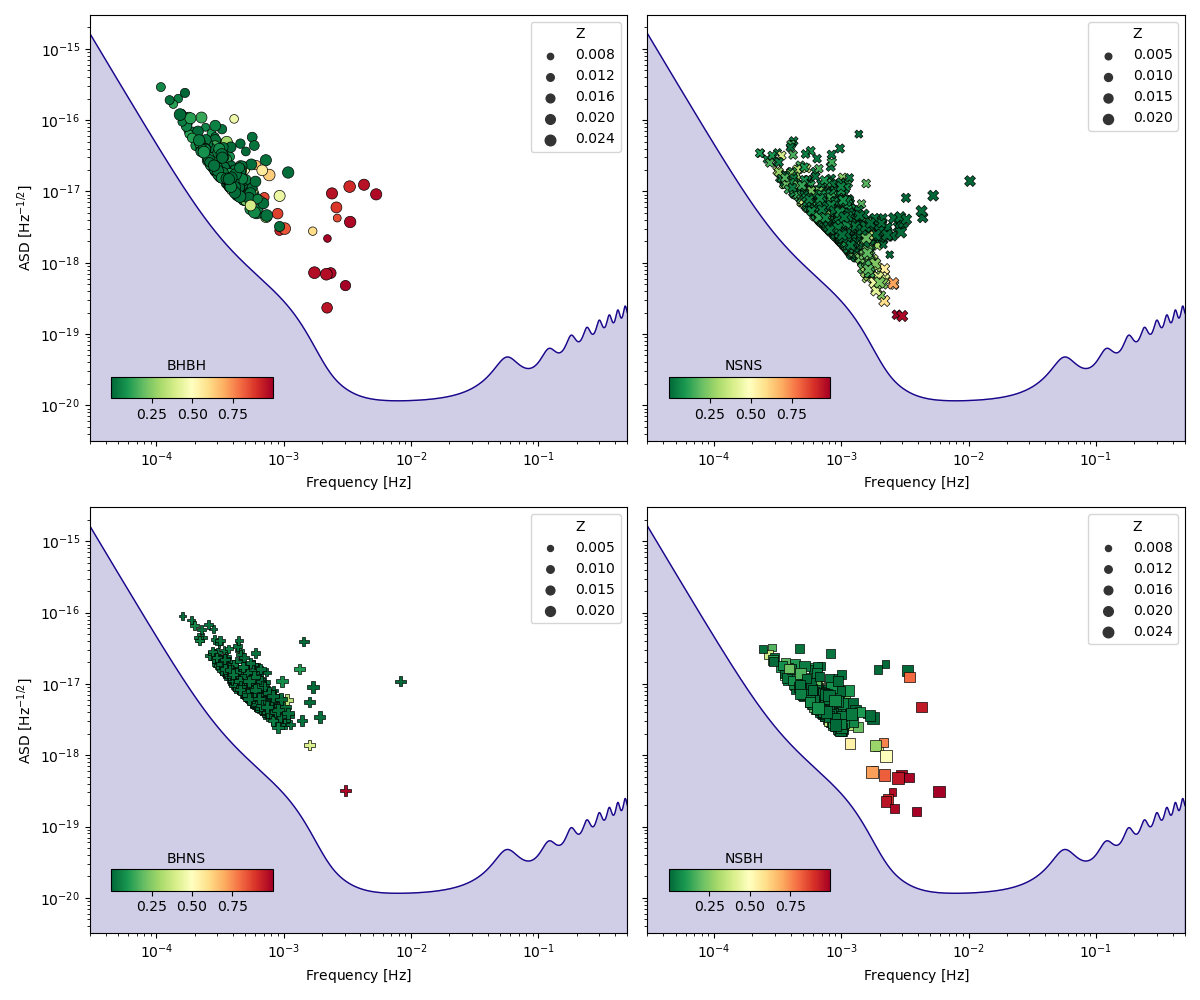
\includegraphics[width=\textwidth]{analysis_data/main_analysis_folder/dco_typewise_snr}
        \caption{Detectable sources' characteristic strain vs. dominant frequency in our simulations are shown on the LISA sensitivity curve. The sources are color-coded based on their eccentricities, green for low and red for high eccentric sources.}
        \label{fig:alldcosnrplotting}
    \end{figure*}

    Using the LEGWORK framework~\cite{wagg2021legwork}, these binaries were than checked for their inspiral phase using the $\interval{evolve}$\footnote{Obtained via COMPAS.} and $\interval{lookback}$\footnote{Obtained via galaxy synthesis.}.
    The difference between lookback and evolution time of a binary was required to be greater than its merger time\footnote{Obtained via LEGWORK framework.}.
    As the number of inspiralling binaries in our study was small compared to the total generated population,\footnote{Due to not using any technique that forces DCO production, e.g., STROOPWAFEL~\cite{Broekgaarden2019}} multiple detections of a single binary object are present in the final output.
    Table~\ref{tab:bhbh-details-table} shows selective details about mass of progenitor and their evolutionary ends for maximum and minimum mass at ZAMS and DCO stages.
    In appendix~\ref{sec:paramter-distribution-across-the-galaxies} we present the number of detection and mean values for selected parameters\footnote{The selected parameters include, $\mone{DCO}$, $\mtwo{DCO}$, $\semaxis{DCO}$, $\ecc{DCO}$, Z, $\interval{evol}$, $\interval{lookback}$, and SNR.} across the hundred instances of MW galaxies.
    The number of detections across all the MW instances came out to be 12758 in total alm

    The predicted distribution of the LISA detectable sources is plotted over its expected sensitivity curve~\cite{Robson2019}, in figure~\ref{fig:alldcosnrplotting}.
    The x-axis shows the dominant frequency, the frequency accumulating the largest SNR, for the eccentric binaries.
    Furthermore, on y-axis we plot the amplitude spectral density (ASD), including the contribution from all harmonics.
    The gap between the detected binaries and the LISA curve in the graph is the SNR criteria, ($\text{SNR}\,>\,7$).
    The size of the points varies with metallicity; high metallic sources have larger shapes and vice versa.
    The color scheme is based on the eccentricity of detected binaries, e.g, the red ones are the most eccentric sources, the yellow ones are mid-eccentric, and the green ones are the sources with low eccentricities.

    Figure~\ref{fig:dcotypemwcomponentdistributioncropped} shows the percentage of different DCOs detected in the \lowalpha, \highalpha and bulge components of the MW instances.
%    In every component, the majority of detections come from BBH pairs.

    \begin{figure}[!h]%
        \centering
        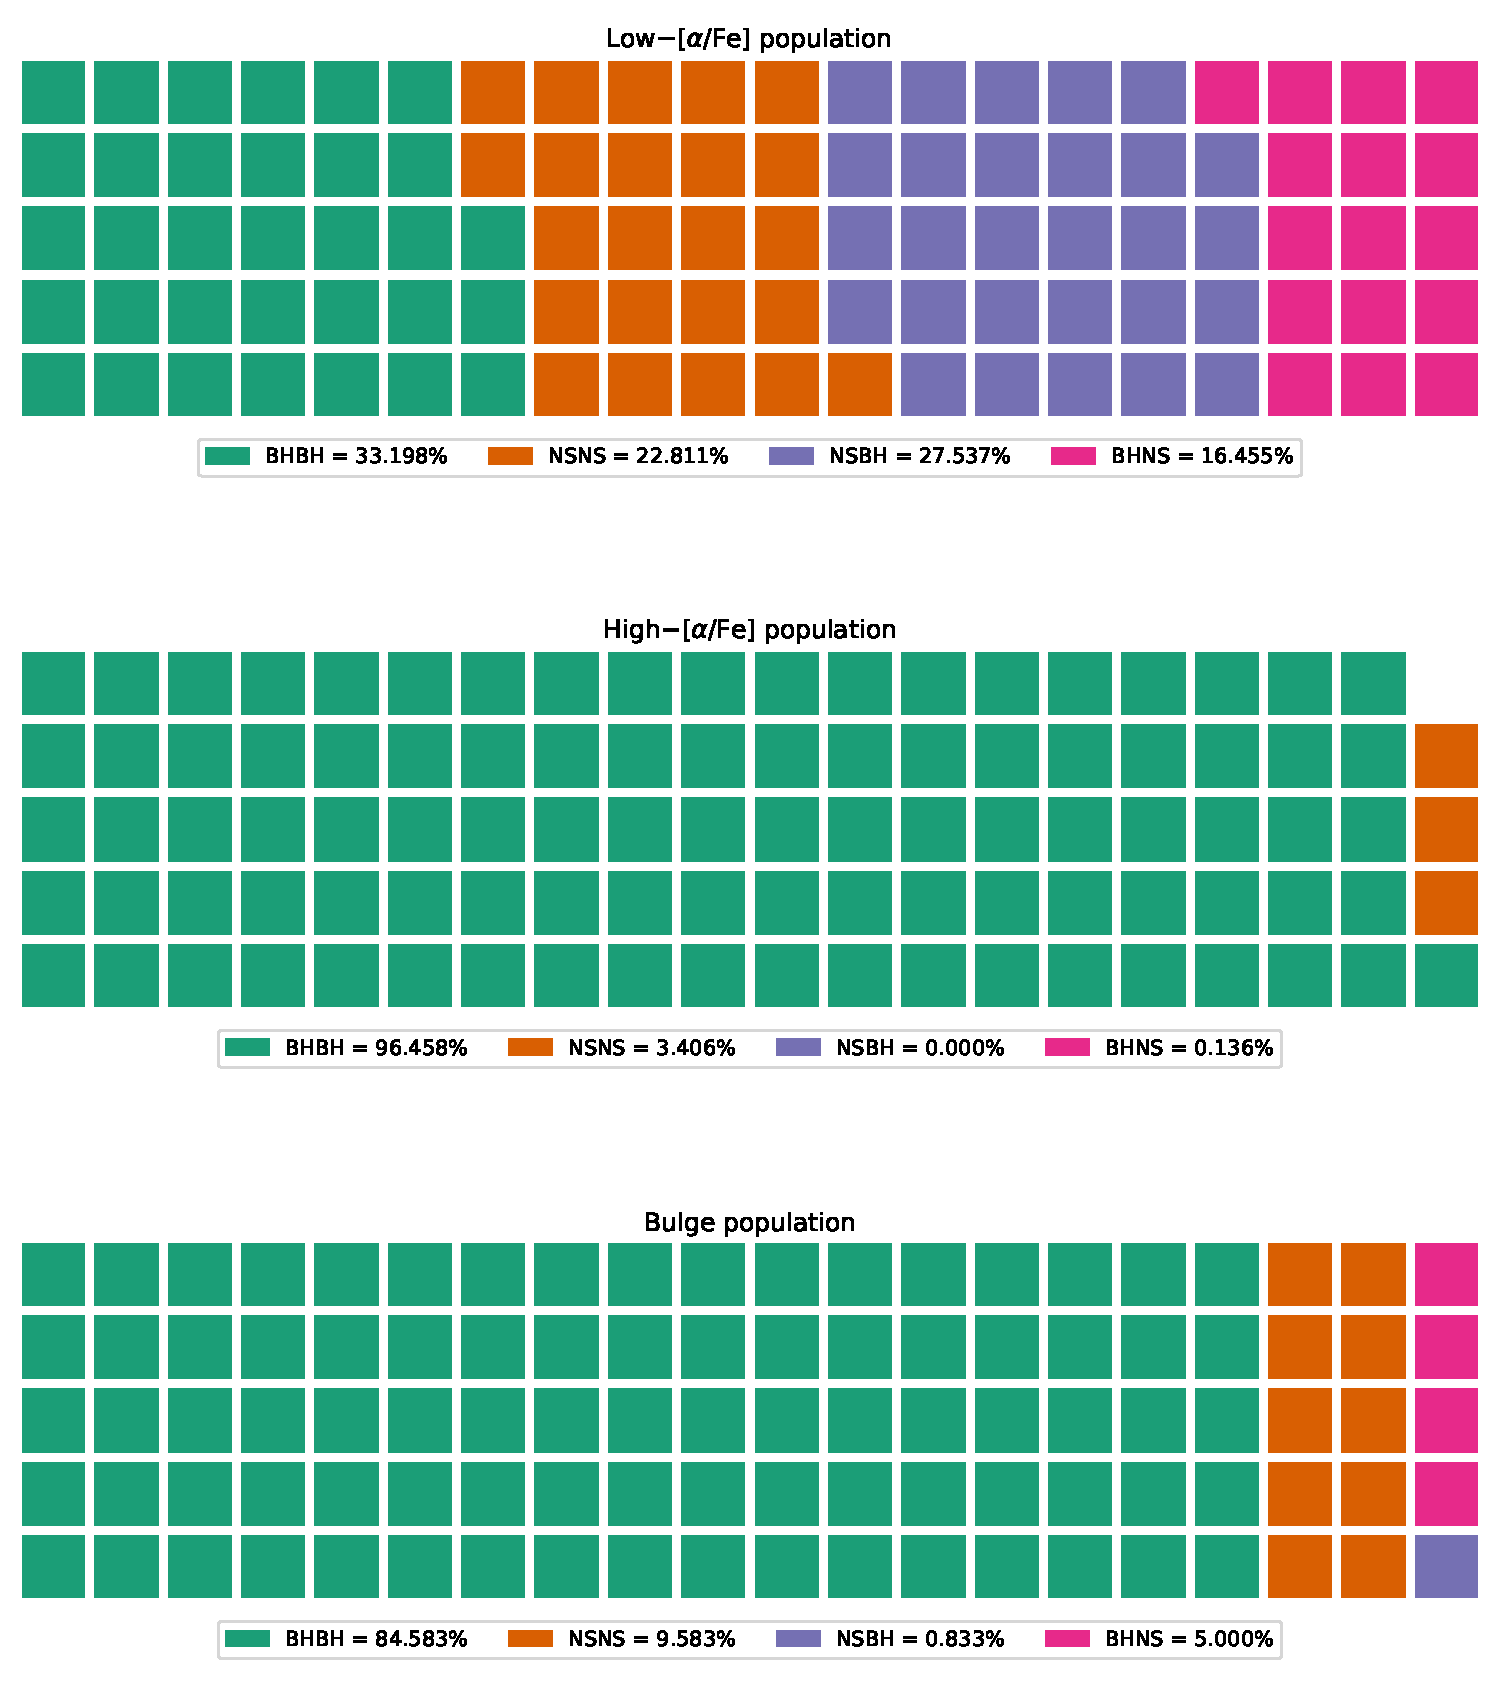
\includegraphics[width=\columnwidth]{analysis_data/main_analysis_folder/dco_type_MW_component_distribution_cropped}
        \caption{Waffle charts showing percentage proportion for DCO type detections in the MW instance components in this study.}
        \label{fig:dcotypemwcomponentdistributioncropped}
    \end{figure}%
    For \lowalpha\ disk, the NSBH pairs have more detections than BHN pairs.
    Contrary to that, NSBH pairs show no detection in \highalpha\ disk, and fractional detection in the bulge, $\sim0.833\%$.
    On the other hand, the BHNS pairs have the lowest detection rate in all three components.

    \begin{figure}[!h]%
        \centering
        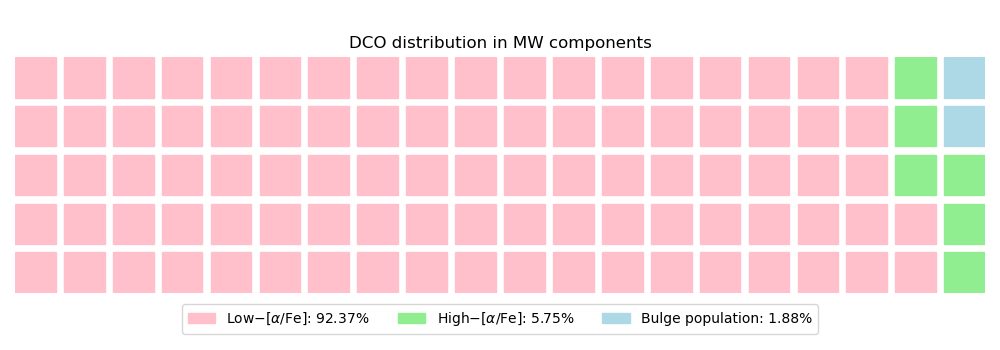
\includegraphics[width=\columnwidth]{analysis_data/main_analysis_folder/dco_type_MW_distribution}
        \caption{Waffle chart showing the total number of detections per MW instance component in this study on the whole.}
        \label{fig:dcotypemwdistribution}
    \end{figure}%

    Figure~\ref{fig:dcotypemwdistribution} shows the percentage of detections in the three components regardless of the DCO type.
    Here we see that majority of the detections are in the \lowalpha\ disk.
    This can be attributed to the biased metallicity value used in this study, $\text{Beta}(5, 80)$.
    These detection percentages do align with the age-metallicity relationship as the bulge is oldest component and thus should have lower metallicity ZAMS stars.
    However, due to the choice of metallicity distribution, these stars were not generated in large numbers.


%	\begin{figure}
%		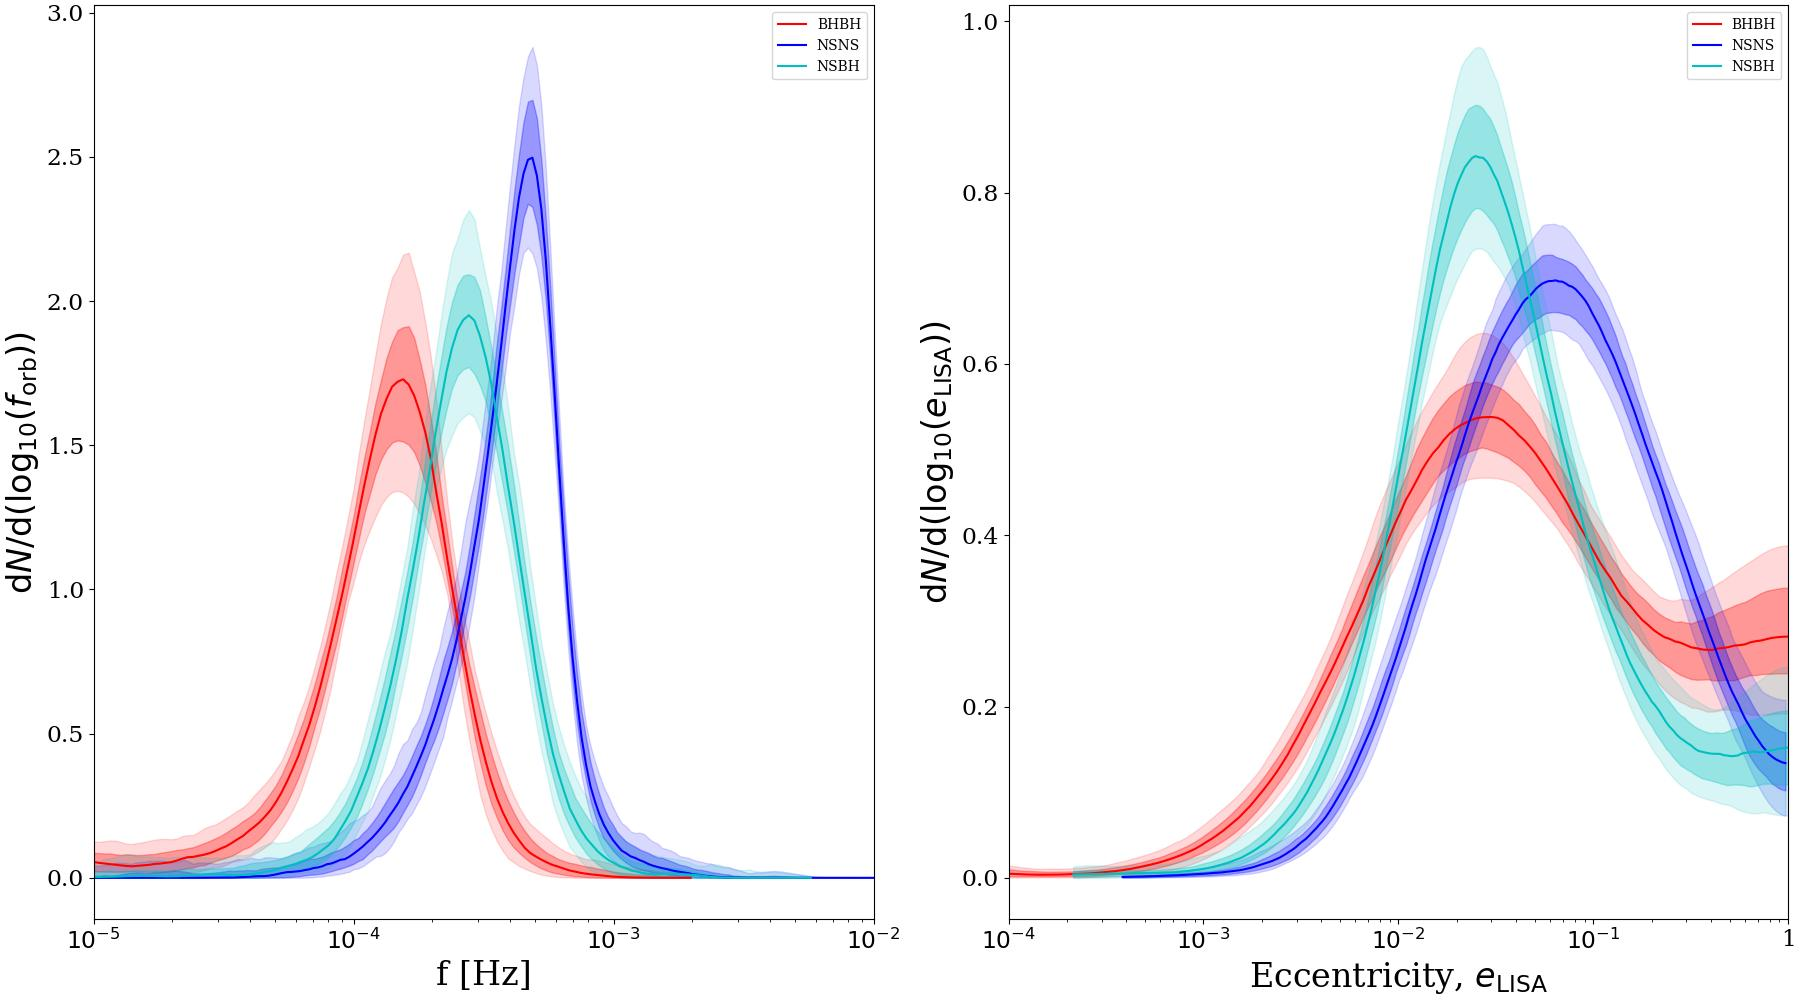
\includegraphics[width=\columnwidth]{images/second}
%		\caption{Caption text.}\label{fig:freq} %--> Fig.1b
%	\end{figure}

%	\subsection{Binary Black Hole pairs (BHBH)}
%	\label{subsec:binary-black-hole-pairs-(bhbh)}
%	Among the detectable BHBH population, 19 pairs have $\ecc{DCO} \geq 0.9$, and a total of 72 pairs having an $\ecc{DCO} \geq 0.75$. On the other end, there are 244 pairs with $\ecc{DCO} \leq 0.25$.

%    Around $3\,\text{mHz}$, some binaries mostly have large eccentricities.
%    These are on the right side of the graph and extend downwards to $10^{-19}$ ASDs. However, there are also some BHBH that are almost circular and emit at high frequency.
%    These sources are in their last stages of merger hence they are spinning fast enough to emit large frequency GW\@.

    The major binary population is concentrated on the left side of the LISA sensitivity curve.
    The peak of concentration around the GW frequency of \textbf{0.12 mHz}.
    The main reason for such a trend can be explained through the eccentricities of the binaries.
    As seen from the figure~\ref{detect}, a large population of our binaries are low eccentric or mid-eccentric.
    There are also binaries having high eccentricities which as mentioned above lie on the right side of the graph.
    The orbit of low eccentric or circular binaries evolves differently than high eccentric binaries.
    After the formation of DCO, most of the low eccentric binaries emit GW in low-frequency bands of LISA as the orbit progresses.
    While DCOs with high eccentricities behave in a completely different way, i.e.\ their orbit decay faster, and they tend to emit GW in the high-frequency LISA detection band.
    Although these are of prime importance in the LISA mission, unfortunately, these are rare.
    Thus, most of the DCOs are at lower frequency regions.

    Fig.~\ref{fig:freq} shows the distribution of the orbital frequency; $f$, and eccentricity at the time of LISA mission; $e$.
    The regions surrounding the individual graphs are the $1\,\sigma$, and $2\,\sigma$ uncertainties which are the variations of the results over 100 random instances of our galaxy.
    We plot this figure using the bootstrapping function~\cite{wagg2021gravitational}.
    The left side of the graph is the orbital frequency distribution.
    It shows peaks of different types of sources i.e. \textbf{0.3mHz, 0.7mHz, 0.99} for BHBH, NSNS, and NSBH\@.
    The reason for such a trend is because of the mass difference as higher mass DCO The distribution is a little negatively skewed.
    As mentioned above, a higher mass DCO at the same distance and eccentricity requires a lower frequency to produce the same signal-to-noise ratio and thus be detected.
    The orbital frequency distributions for BHBHs, BHNSs, and NSNSs (figure, 3a) peak at progressively increasing
    frequencies as mentioned in section 3.1.
    The distributions appear nearly symmetric, but closer inspections show that the left-hand side is more populated, which can be seen most clearly in the curve for the BHBHs.
    This is due to the contribution of highly eccentric binaries, which are most abundant in the BHBH population.
    These systems are still detectable by LISA, despite their low orbital frequency, as the high eccentricity means that the majority of the GW signal is emitted at higher harmonics, where LISA is more sensitive.

    We can also observe the peaks for high chirp mass systems have peaks in the low-frequency detection region, as they emit the waves in lower frequency.
    Hence, this is another way to differentiate sources.
    Hence, the BHBH pairs have the most eccentric pairs having the highest average eccentricity and $\langle M_c\rangle$.

%    \subsection{Detections in Components}\label{subsec:detectionetections-in-components}
%    Our simulated galaxy comprises three components; Low $\alpha$ disc, High $\alpha$ disc, and Bulge.
%    Figure~\ref{fig:pie1} describes the average distribution of detectable sources in these components.
%    The average total number of detections are in shown in the middle.
%    BHBH, having a significant number of detections, is equally distributed in the low$-\alpha$ disc and high$-\alpha$ disc, while the rest have slightly more detections in the latter than prior.
%    Bulge has the least number of detected DCOs.
%    Thus, there is a high probability for LISA to detect GW sources in the two components.
%
%    \begin{figure}
%        \centering
%        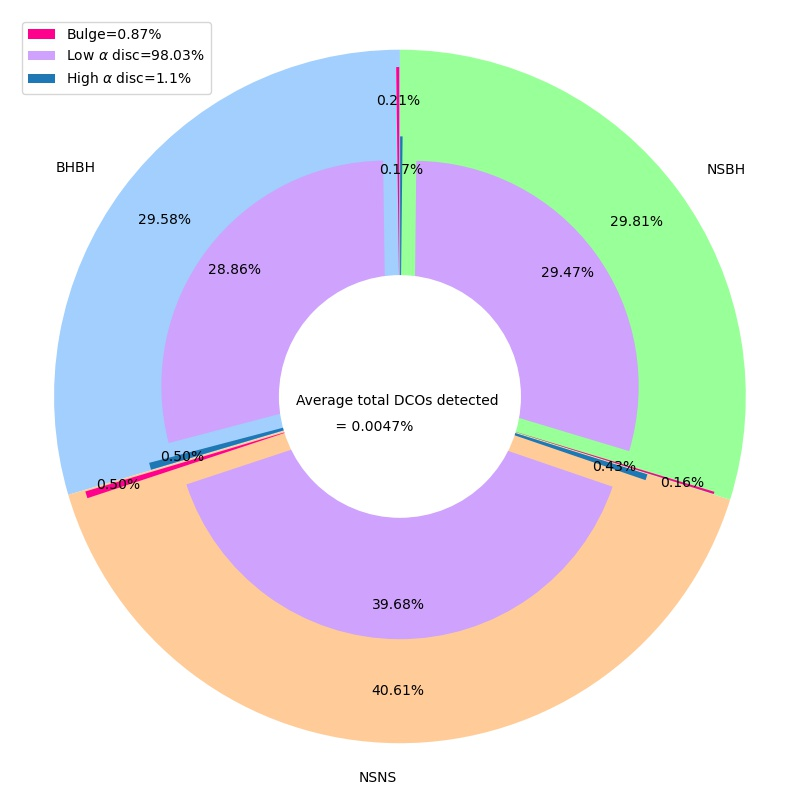
\includegraphics[width=\linewidth]{images/pie_chart}
%        \caption{Average detectable sources distribution in three components of simulated milky way}
%        \label{fig:pie1}
%    \end{figure}

    \subsection{Maximum distance}\label{subsec:maximum-distance}
    For each DCO, there is a horizon distance i.e., the maximum distance up to which the DCO may be detectable in
    LISA. This is calculated using the inverse relationship between SNR ($\rho$) and distance~\cite{Lau2020},
    \begin{equation}
        \label{eq:eq1}
        d_\text{max}=\frac{\rho(d\,=\,1\,\text{kpc})}{\rho_\text{min}}
    \end{equation}

    Where $\rho_{\min}$ is the minimum value of SNR below which the source is not detectable.
    We keep the detection threshold at $\rho_{\min}\,=\,7$, and $\rho(d\,=\,1\,\text{kpc})$ is SNR of the source if it was at $1\,\text{kpc}$ distance from the detector.
    We calculated the SNR of all the detected sources at \SI{1}{\kpc} distance using the python package LEGWORK~\cite{wagg2021legwork}.
    Afterward, their maximum distances $(d_{\max})$ were calculated.

    Figure~\ref{fig:dmax} shows the maximum distances for all the detected sources.
    The top shows $d_{\max}$ for BHBH, and NSNS while the bottom has NSBH and BHNS\@.
    These are calculated for all the LISA band frequencies.
    The black line shows the average maximum distance for all the types.
    The LISA sensitivity curve is also overlaid on the graph as a blue line.

    BHBH, being the dominant source can be observed to an average distance of more than \SI{1e5}{\kpc}.
    NSBH and BHNS have almost the same average $d_{\max}$ i.e between \SI{1e3}{\kpc} and \SI{1e4}{\kpc} while NSNS has peak at $\sim\,$\SI{1e3}{\kpc}.
    The red dotted lines illustrate some known galaxies to have a better understanding of distances.
    Hence, BHBH can be discovered as far as Hoag's Object, NSNS in M31, and both BHNS and NSBH are far from M31 but much below Hoag's Object.


    Almost all the highest values of average $d_{\max}$ of four types are around a \textbf{certain frequency} i.e., if a source has \textbf{certain orbital frequency} then it can be detected to its maximum detection distance.
    It can be observed through the LISA overlay that this frequency lies in the area where the detector is most sensitive.
    Hence, if a source emits in the frequency region of the highest sensitivity of LISA, then it will be detected at a maximum distance.

    \begin{figure}
        \centering
        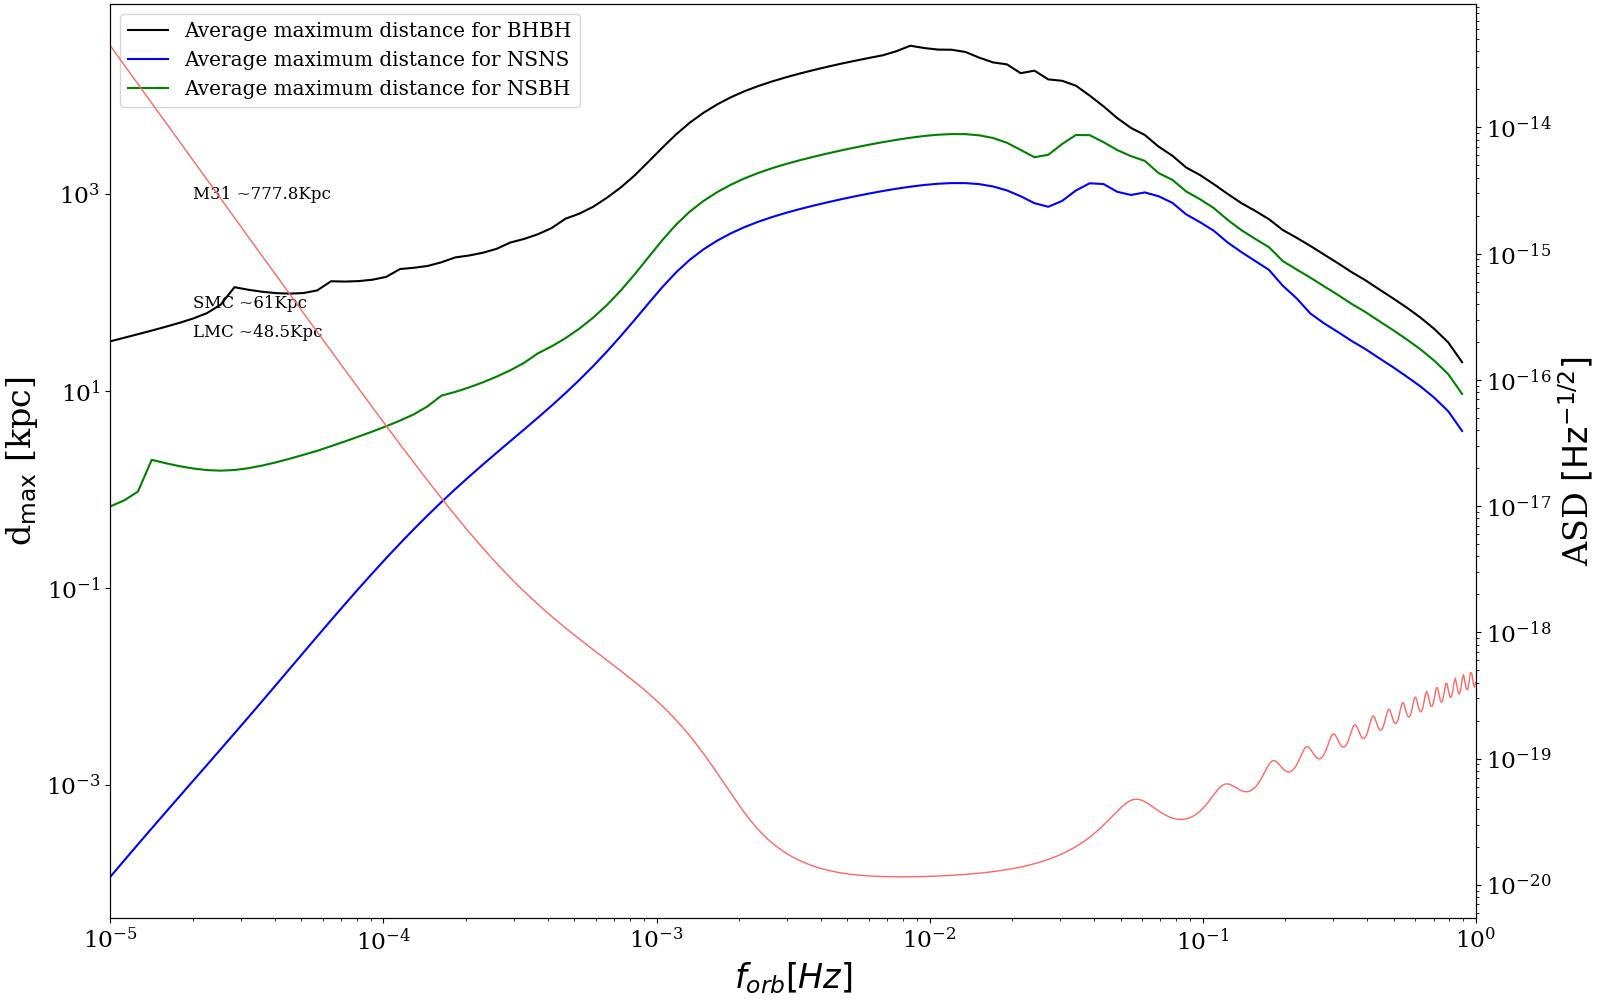
\includegraphics[width=\linewidth]{images/DMAX}
        \caption{Maximum distances for all of the different types of DCO. The average maximum distance is
        shown through a black line while the blue line shows the overlaid LISA sensitivity curve}
        \label{fig:dmax}
    \end{figure}


    \section{Comparative analysis}
    \label{sec:comparative-analysis}
    In this section, we will deal with the comparative study of our eccentric binary data set $(\aleph_1)$ with circular binary data set, $(\aleph_2)$.
    In order to fairly compare the outputs of the two data sets, given only the difference of eccentricity, we make use of the seed numbers provided in $\aleph_1$ data set.
    With the exception of SN kick parameters and eccentricity, all the other parameters were kept the same as in $\aleph_1$.
    We evolved the binaries consistent with the method described in this paper.
    
    \subsection{Hubble Merger Rate} 
    After running the simulations, we obtained 9751 DCO pairs ($\sim0.09751\%$). Out of these, only 5178 ($\sim53.1022\%$) were able to merge within Hubble time. Table~\ref{tab:dco_details0e} shows the proportion of DCO merger for each DCO type for $\aleph_2$ data set.
    
    \begin{table}[!h]%
		\centering
		%        \resizebox{\columnwidth}{!}{
		\begin{tabular}{@{}cccc@{}}
			\toprule
			\multirow{2.5}{*}{BHBH} & \multirow{2.5}{*}{NSNS} & \multicolumn{2}{c}{BHNS} \\ \cmidrule(l){3-4}
			&           & NSBH    & BHNS     \\ \midrule
			189/285 & 4438/8605 & 193/293 & 385/568 \\ \bottomrule
		\end{tabular}%
		%    	 }
		\caption{Number of DCOs merged within Hubble time vs total DCOs formed by the COMPAS suite for circular binary data set.}
		\label{tab:dco_details0e}
	\end{table}%
	Like the $\aleph_1$ data set, the highest merging rate for $\aleph_2$ comes from BHBH as well ($\sim66.32\%$), followed by BHNS pairs $(\sim65.87\%)$, NSBH $(\sim63.03\%)$ and lastly, NSNS dco type $(\sim51.57\%)$.

	\subsection{Effects of eccentricity}	
	A total of 140 seeds were found common between the two data sets.
    Out of these 140 seeds, 105 were found to evolve to the same final stage before merging. The binaries with common and diverging final evolutionary stages are shown in figure~\ref{fig:dcotypedivergenceintwodatasets}.
    The lesser number of diverging cases indicate that the ZAMS eccentricity might not play as much of a bigger role in the evolution of the binaries.
    
    \begin{figure*}[!h]%
    	\centering
    	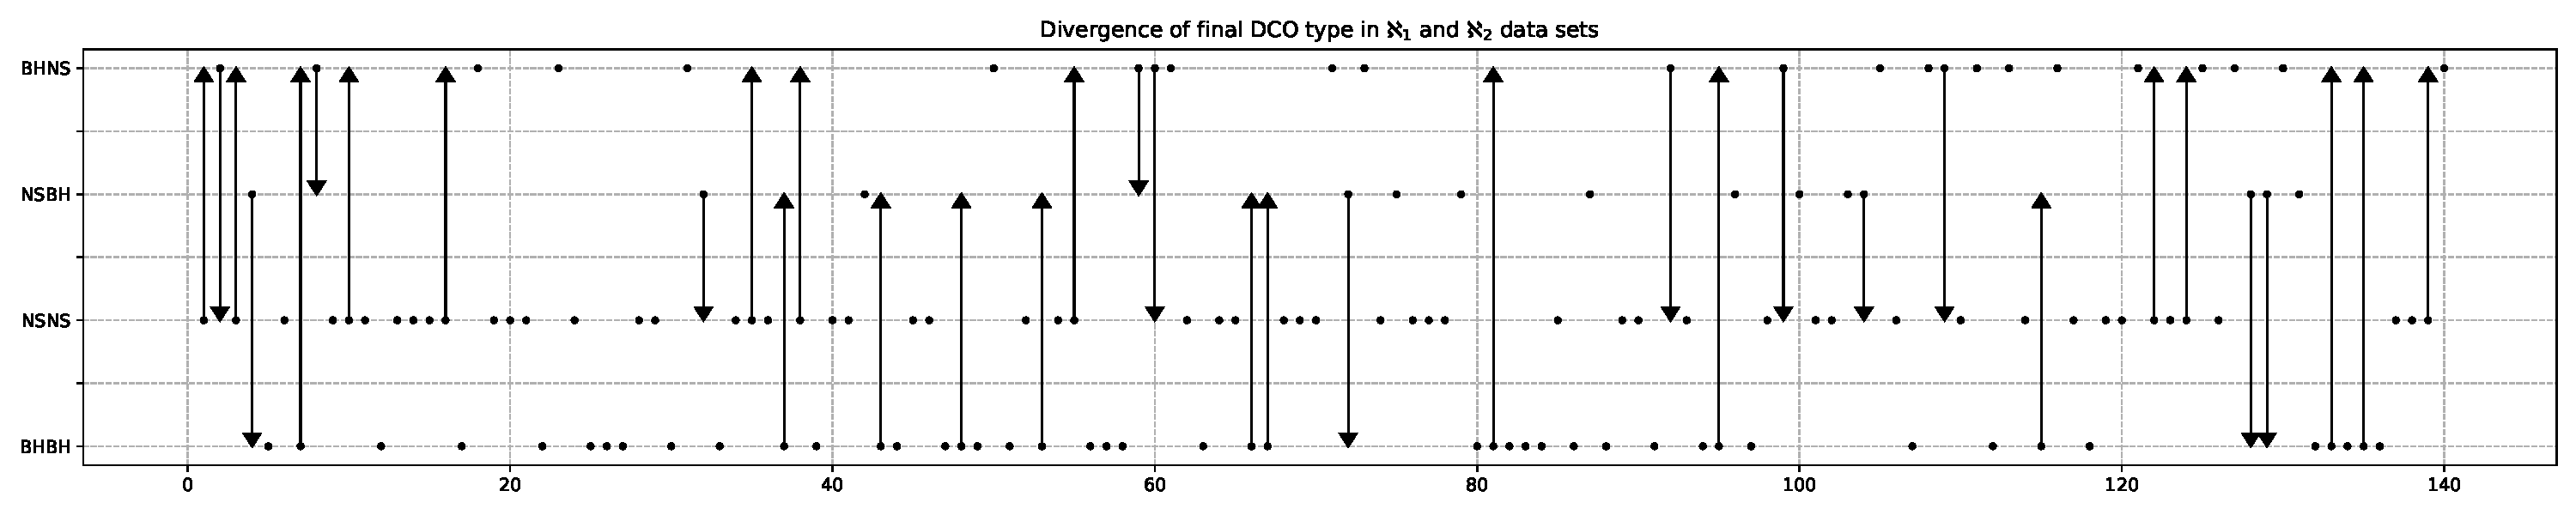
\includegraphics[width=\textwidth]{analysis_data/dcotype_divergence_in_two_datasets}
    	\caption{Plot showing the change in DCO ending states for the common seed numbers from $\aleph_1$ and $\aleph_2$ data sets. The direction of arrows shows the change in the DCO type from $\aleph_1$ and $\aleph_2$ data set. The binaries that didn't change the DCO type after evolution are represented by a filled dot.}
    	\label{fig:dcotypedivergenceintwodatasets}
    \end{figure*}%
    
	
    \subsection{Detection rates}\label{subsec:detectionetection-rates}
    The prediction for VE is a total of 136 detections in a 4 years LISA mission.
    A decrease in the detection rate is observed for E0 which is detected in a 4 years LISA mission.
    As there is no difference in any parameter other than eccentricity, then it is surely the root cause of the decline in detections.

    The difference in different types of sources is shown in the pie chart in which there is a clear reduction in the detected sources. \textbf{Explain the pie chart more}

    %\begin{figure}
    %    \centering
    %    \includegraphics[width=\linewidth]{pie_e0_evar.jpg}
    %    \caption{Comparison of detection rate in VE and E0.}
    %    \label{pie}
    %\end{figure}

    \subsection{Model variation: To be added somewhere else,}
    \label{subsec:model_variation}
    In a number of previous works, $e_\text{ZAMS}$ was taken as zero~\cite{Vigna2018, Barrett2018, Lau2020, Broekgaarden2021, wagg2021gravitational}.
    The main reason for this assumption is that they argue that eccentricity at ZAMS is not likely critical for predicting detection rates as they deal with post-interaction binaries and their orbital eccentricities become zero after mass transfer~\cite{Hurley2002}. %, de2015merger}).
    To test the accuracy of this assumption, we simulate another population with the same parameters.
    The only change is that $e_\text{ZAMS}$ of the binaries is left to be varied by the COMPAS suite.
    We compare the difference in detection rates and properties of the two models and give our conclusion.


    \section{Discussion and Future work}\label{sec:df}
    \ifCLASSOPTIONcaptionsoff
    \newpage
    \fi

    \cleardoublepage
    \bibliographystyle{others/apj}
    \bibliography{reference}

    \cleardoublepage
    %	\onecolumn
    \appendices
    \section{Settings for using COMPAS}
\label{sec:appA}
To generate a binary system in COMPAS, we require the following parameters as discussed earlier,
\begin{itemize}
    \item mass of primary star $(\mone{ZAMS})$,
    \item mass of secondary star $(\mtwo{ZAMS})$,
    \item semi-major axis of the orbit $(\semaxis{ZAMS})$,
    \item random seed $(\o)$
    \item remnant mass prescription,
    \item eccentricity of the orbit $(\ecc{ZAMS})$, and
    \item metallicity of the stars $\left(Z\right)$.
\end{itemize}

We've discussed the first four parameters in the main text, here we will discuss the selection of eccentricity and metallicity values.

\subsection{\textbf{Eccentricity}}
\label{subsec:eccentricity}
In order to evaluate whether the initial eccentricity affects GW emission at the end stages of the DCO, we generate two identical data sets.
For the primary data set, we chose the eccentricity value to be varied between 0 and 1.

For the secondary data set, we assumed all the binaries to have circular orbits.
For cross-checking purposes we made sure to use the same seed numbers when generating the second data set that were used with the primary data set.
This enabled us to check the effects of initial eccentricity on the formation of double compact objects.
For the selection of eccentricity, the power law and gamma distribution were also considered (see, figure~\ref{fig:pl_distribution} and~\ref{fig:gamma_distribution} respectively).

\subsubsection*{\textbf{Power law distribution}} The random values for metallicity were generated using the power law distribution given below,
\begin{equation}
    f(x, a) = ax^{(a-1)}
    \label{eq:powerlaw_distribution}
\end{equation}
where $a$ is the index of the power law distribution.\footnote{\url{https://docs.scipy.org/doc/scipy/reference/generated/scipy.stats.powerlaw.html}}
Figure~\ref{fig:pl_distribution} shows the plot for the probability density function (PDF) of the power law with $a \in [1, 2]$.
Although the distribution can produce higher values, it does not suppress the lower values so this distribution was discarded.
\subsubsection*{\textbf{Gamma distribution}}
For the probability density function for gamma distribution,\footnote{\url{https://docs.scipy.org/doc/scipy/reference/generated/scipy.stats.gamma.html}} we use the following form,
\begin{equation}
    f(x, a) = \frac{x^{a-1}\exp(-x)}{\Gamma(a)}
    \label{eq:gamma_distribution}
\end{equation}
for $x\geq 0$ and $a > 0$.
Here, $a$ is the shape factor, and $\Gamma$ is the gamma function, such that $\Gamma(a) = (a-1)!$.
Similar to the power law distribution, the gamma distribution was not a good selection for the values of metallicity that were required for this study.
\begin{minipage}[r]{0.48\textwidth}
    \centering
    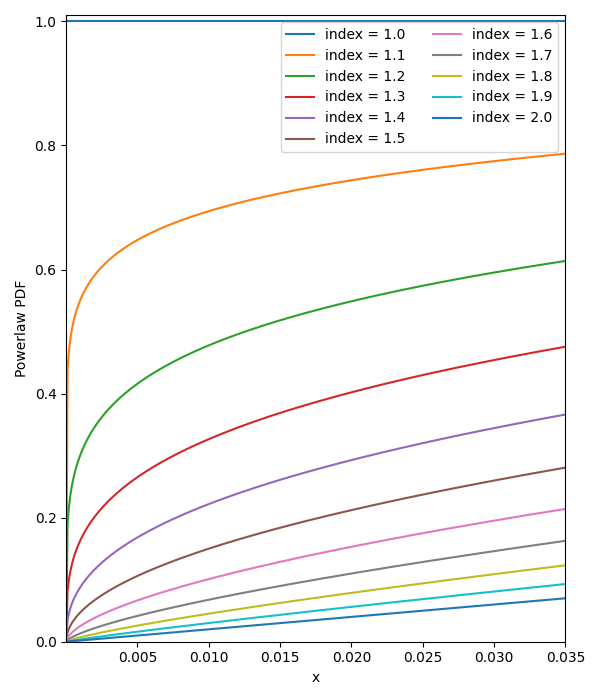
\includegraphics[width=\textwidth]{images/powerlaw}
    \captionof{figure}{Power law distribution}
\end{minipage}

\,\\\subsubsection*{\textbf{Beta distribution}}
For the beta distribution, we use the following form,
\begin{equation}
    f(x, a, b) = \frac{\Gamma(a+b)x^{a-1}(1-x)^{b-1}}{\Gamma(a)\Gamma(b)}
    \label{eq:beta_distribution}
\end{equation}
For $0 \leq x \leq 1, a > 0, b > 0$ and $\Gamma$ is the gamma function.\footnote{\url{https://docs.scipy.org/doc/scipy/reference/generated/scipy.stats.beta.html}}

Figure~\ref{fig:beta1} shows the beta distribution with a fixed $\beta=80$.
Similarly, figure~\ref{fig:beta2} shows the beta distribution with a fixed $\alpha=5$.
For our case, we selected $\text{Beta}(5, 80)$ as our distribution of choice for metallicity and generated $10^7$ values between the COMPAS limits $10^{-4} < z < 0.03$. %The same value for metallicity was used for both stars as different metallicity scenario is highly unlikely.

\begin{figure}[!ht]%
    \centering
    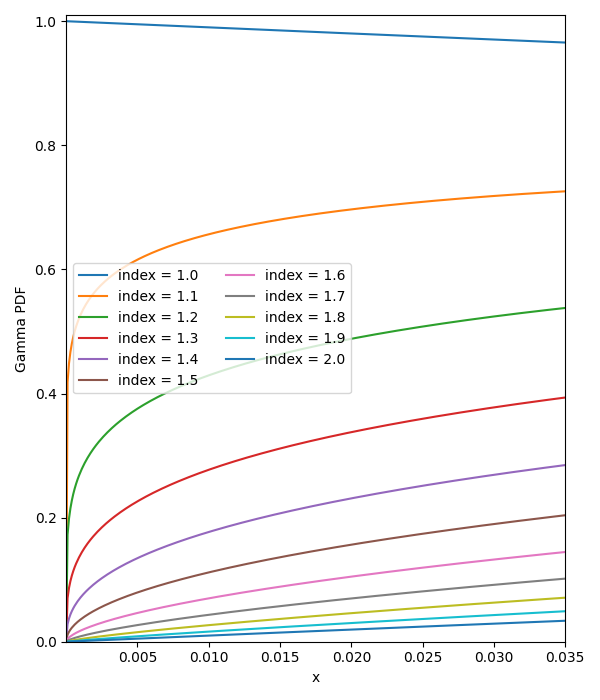
\includegraphics[width=\linewidth]{images/gamma}
    \caption{Gamma distribution with $1 \leq a \leq 2$.}
    \label{fig:gamma_distribution}
\end{figure}%
\begin{figure}[!ht]%
    \centering
    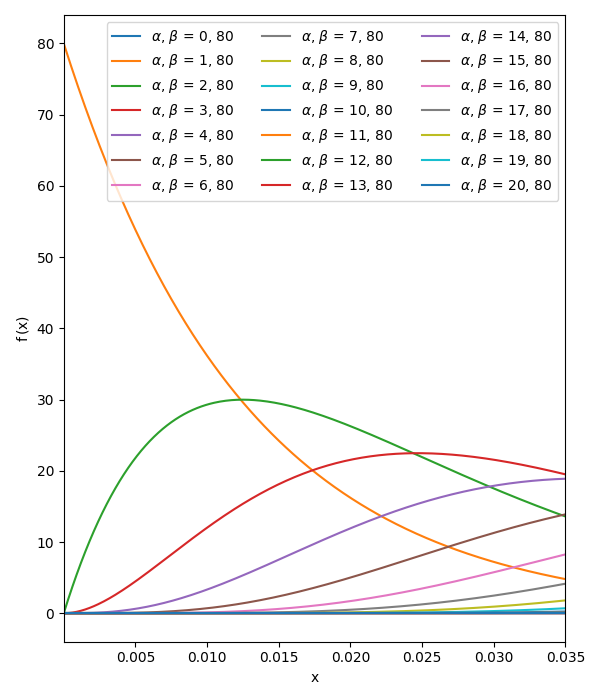
\includegraphics[width=\linewidth]{images/beta1}
    \caption{Beta distribution with varying $\alpha$ and fixed $\beta$ parameter.}
    \label{fig:beta1}
\end{figure}%
\begin{figure}[!ht]%
    \centering
    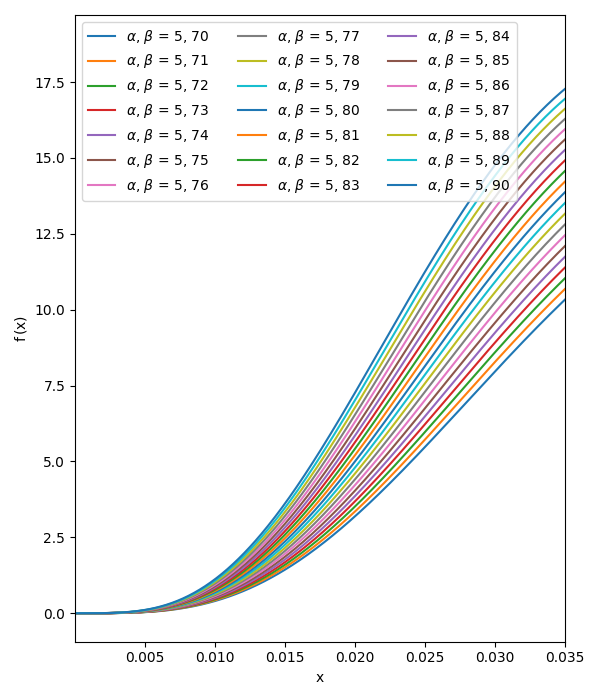
\includegraphics[width=\linewidth]{images/beta2}
    \caption{Beta distribution with fixed $\alpha$ and varying $\beta$ parameters.}
    \label{fig:beta2}
\end{figure}%

\subsection{\textbf{Metallicity}}
\label{subsec:metallicity}
One of the major challenges in generation of the stellar binaries for this study was the selection of a distribution which will result in stars at the higher end of COMPAS metallicity boundary, $z = 0.03$.
A power-law, gamma, and beta distributions were selected to try and simulate the required metallicity distribution.
In the following section, we discuss the selected distributions briefly,
    \newpage
    \section{Milky way Model}
\label{sec:milky_way}
In this section, we will briefly outline the milky way galaxy model used in this study.
The model is developed by~\cite{wagg2021gravitational} and makes use of the galaxy's enrichment history by taking
into account the metallicity-radius-time relationship~\cite{Frankel2018}.
It uses a separate star formation history and spatial distribution for the \lowalpha, \highalpha\ discs, and bulge in the galaxy.

\subsection{Star formation rate}
\label{subsec:star_formation_rate}
The star formation rate for both the \lowalpha\ and \highalpha\ disks is expressed as,
\begin{equation}
    p(\tau) \propto \exp\left(-\frac{\tau_m - \tau}{\tau_\text{SFR}}\right),
    \label{eq:star_formation_rate_equation}
\end{equation}
where $\tau$ is the time difference between the star's ZAMS stage and today.
The age of milky way galaxy, $\tau_m$, is taken as \SI{12}{\giga\yr}, and the star formation rate as, $\tau_\text{
    SFR}\ $= \SI{6.8}{\giga\yr}.
The star-forming period of \lowalpha\ and \highalpha\ discs were taken as \SIrange{0}{8}{\giga\yr} and \SIrange{8}{12}{\giga\yr} respectively.
The model adopts \SIrange{6}{12}{\giga\yr} as the star-forming period of the bulge~\cite{Bovy2019}.

\subsection{Radial distribution}
\label{subsec:radial_distribution}
The radial distribution of stars within the milky way galaxy was performed using the following expression,
\begin{equation}%
    p(R) = \exp\left(-\frac{R}{R_d}\right)\frac{R}{R_d^2}
    \label{eq:radial_distribution_of_stars}
\end{equation}%

However, a different scale length, $R_d$, was chosen for each component of the galaxy.
For \lowalpha, the model uses $R_\text{exp}(\tau)$ as the scale length~\cite[Eq 6]{Frankel2018}, where

\begin{equation}%
    R_\text{exp}(\tau) = 4\,\text{kpc}\left[1 - \alpha_{R_\text{exp}}\left(\frac{\tau}{8\,\text{Gyr}}\right)\right],
    \label{eq:exponential_radius_equation}
\end{equation}%
with the value of inside-out growth parameter, $\alpha_{R_\text{exp}}$, as 0.3. For \highalpha\ disc and bulge, the value of scale length was chosen as $(1/0.43)\,$\si{\kpc} and \SI{1.5}{\kpc} respectively.

\subsection{Vertical distribution}
\label{subsec:vertical_distribution}
The model employs a similar method of single exponent expression with varying scale height parameters for the vertical distribution as well.
The exponential expression used is,
\begin{equation}
    p(|z|) = \frac{1}{z_d}\exp\left(-\frac{z}{z_d}\right),
    \label{eq:vertical_distribution_of_stars}
\end{equation}
where $z$ here is the vertical displacement from the galactic plane.
The scale height parameter, $z_d$, for \lowalpha, \highalpha\ and bulge was taken as \SI{0.3}{\kpc}~\cite{McMillan2011}, \SI{0.95}{\kpc}~\cite{Bovy2016}, and \SI{0.2}{\kpc}~\cite{Wegg2015} respectively.

\subsection{Metallicity-radius-time relationship}
\label{subsec:metallicity_radius_relationship}
The MRT relationship plays an important part, both in the galaxy model and later on in the placement of DCOs within the galaxy as well.
The model makes use of~\cite[Eq. 7]{Frankel2018},
\begin{equation}
    \feh(R,\tau) = F_m + \nabla\feh R - \left(F_m + \nabla\feh R_{\feh=0}^{\text{now}}\right) f(\tau)
\end{equation}
For each point generated, if the value of metallicity produced by the MW model was less or greater than the limits defined by COMPAS\footnote{0.0001, 0.03} it was changed to a uniformly drawn random number between $\text{COMPAS}_\text{min} - \text{ZSOLAR}$ and $\text{ZSOLAR} - \text{COMPAS}_\text{max}$ respectively.
\subsection{Galaxy synthesis}
\label{subsec:galaxy_synthesis}
For the synthesis of an instance of the Milky Way galaxy, the model described previously samples the following parameters,
\begin{equation*}
    \theta_i = \{\tau, D, z, \text{component}\},
\end{equation*}
where $\tau$ is the look-back time for the binary, $D$ is the distance from Earth, $z$ is the metallicity, and `component' is the component of the galaxy in which the binary resides.\footnote{One of the three, \lowalpha\ disc, \highalpha\ disc, or bulge.}
The parameters are generated for $i = 1, 2, 3, \ldots$, $N_\text{GAL}$, where $N_\text{GAL} = 100$.
    \newpage
    \section{Parameter distribution across the galaxies}
\label{sec:paramter-distribution-across-the-galaxies}
\subsection{Binary Black Holes}
\begin{figure}[!h]
    \centering
    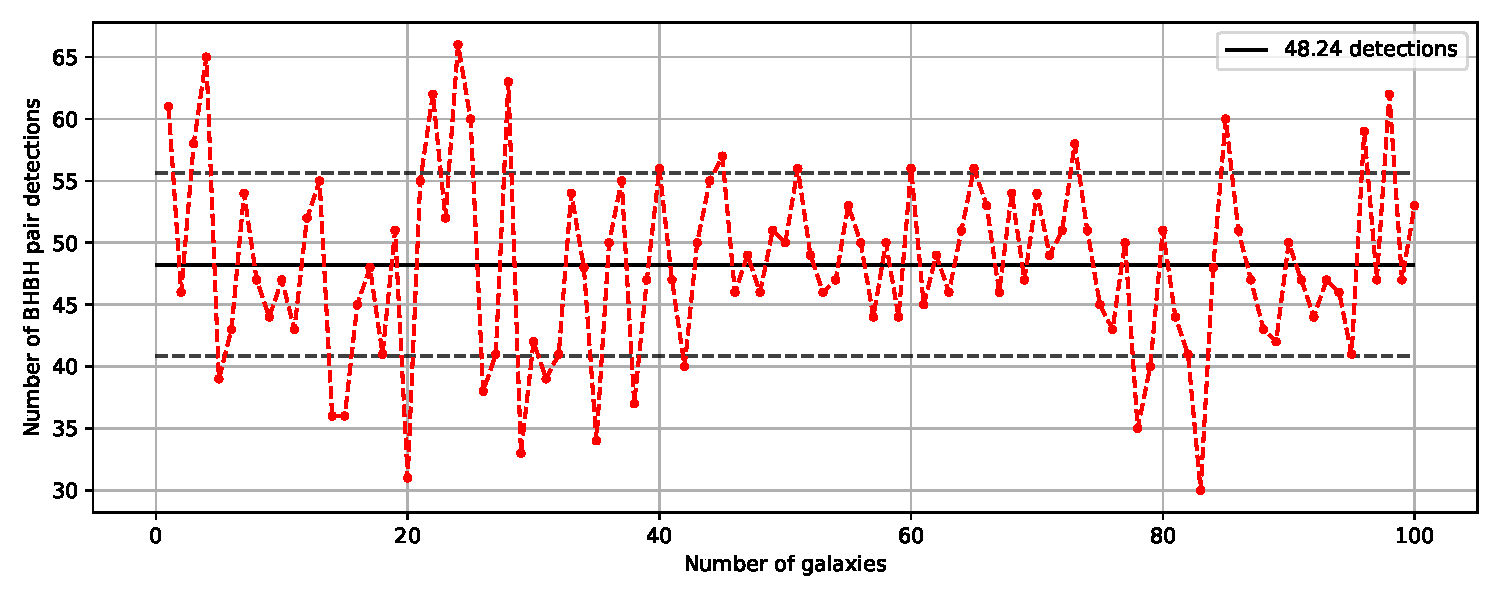
\includegraphics[width=\columnwidth]{analysis_data/main_analysis_folder/BHBH_n_detections}
    \caption{Number of BHBH pair detection per galaxy instance. On average, a total of $\sim$48 pairs per galaxy were detected in this study.}
    \label{fig:bhbhndetections}
\end{figure}

\begin{figure}[!h]
    \centering
    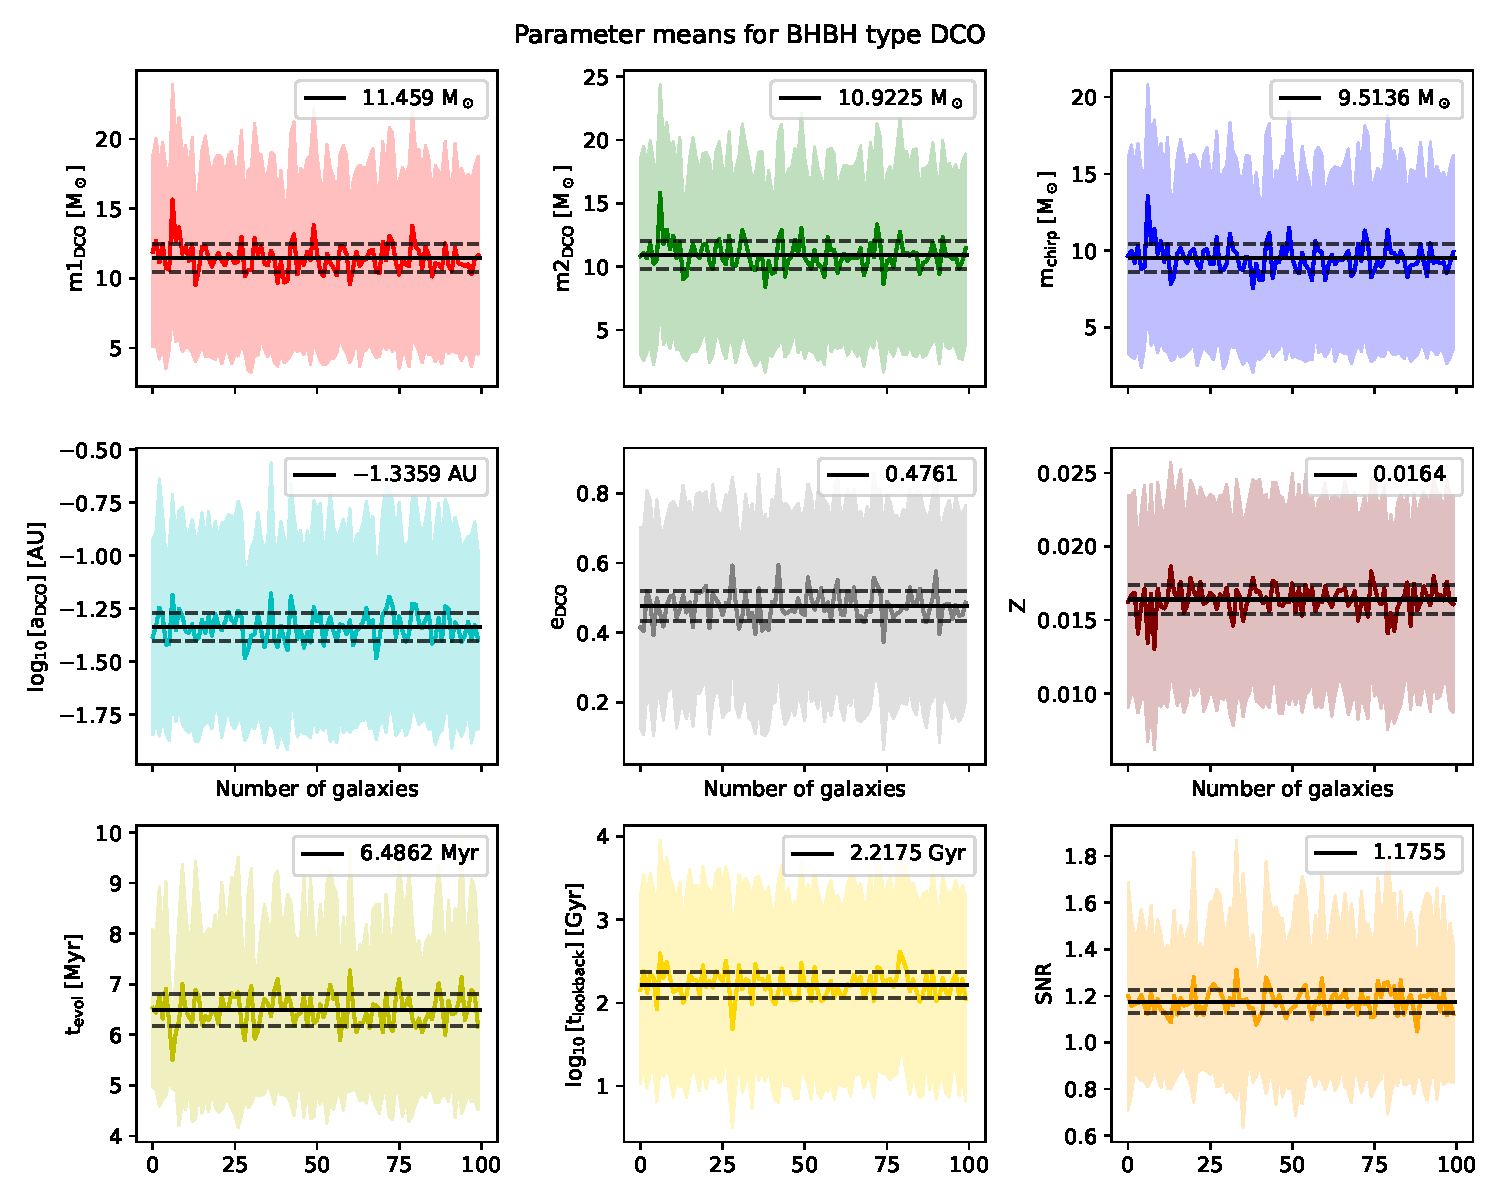
\includegraphics[width=\columnwidth]{analysis_data/main_analysis_folder/BHBH_n_galaxy_mean_plot}
    \caption{The mean and standard deviation for selected parameters in every galaxy is plotted against the galaxy number. An overall measure of mean and standard deviation of all the galaxies is also shown for selected parameter with a black solid and dashed lines respectively.}
    \label{fig:bhbh_n_galaxy_mean_plot}
\end{figure}

\subsection{Binary Neutron Stars}
\begin{figure}[!h]
	\centering
	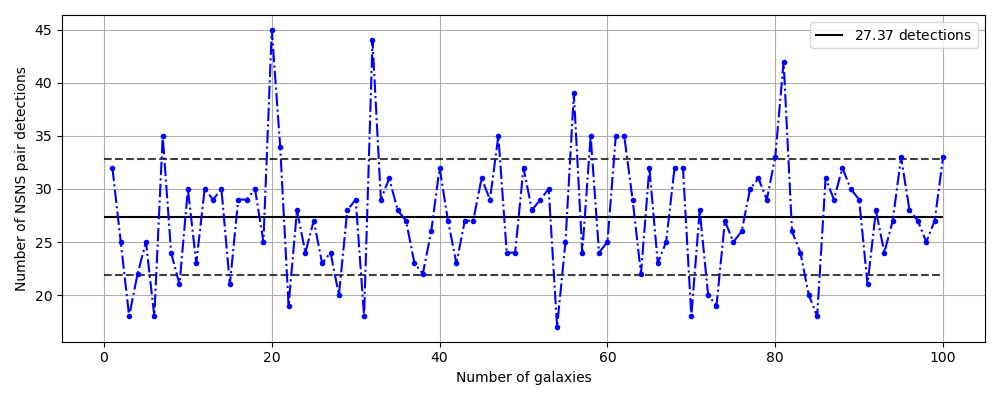
\includegraphics[width=\columnwidth]{analysis_data/main_analysis_folder/NSNS_n_detections}
	\caption{Number of NSNS pair detection per galaxy instance. On average, a total of $\sim$27 pairs per galaxy were detected in this study.}
	\label{fig:nsnsndetections}
\end{figure}

\begin{figure}[!h]
	\centering
	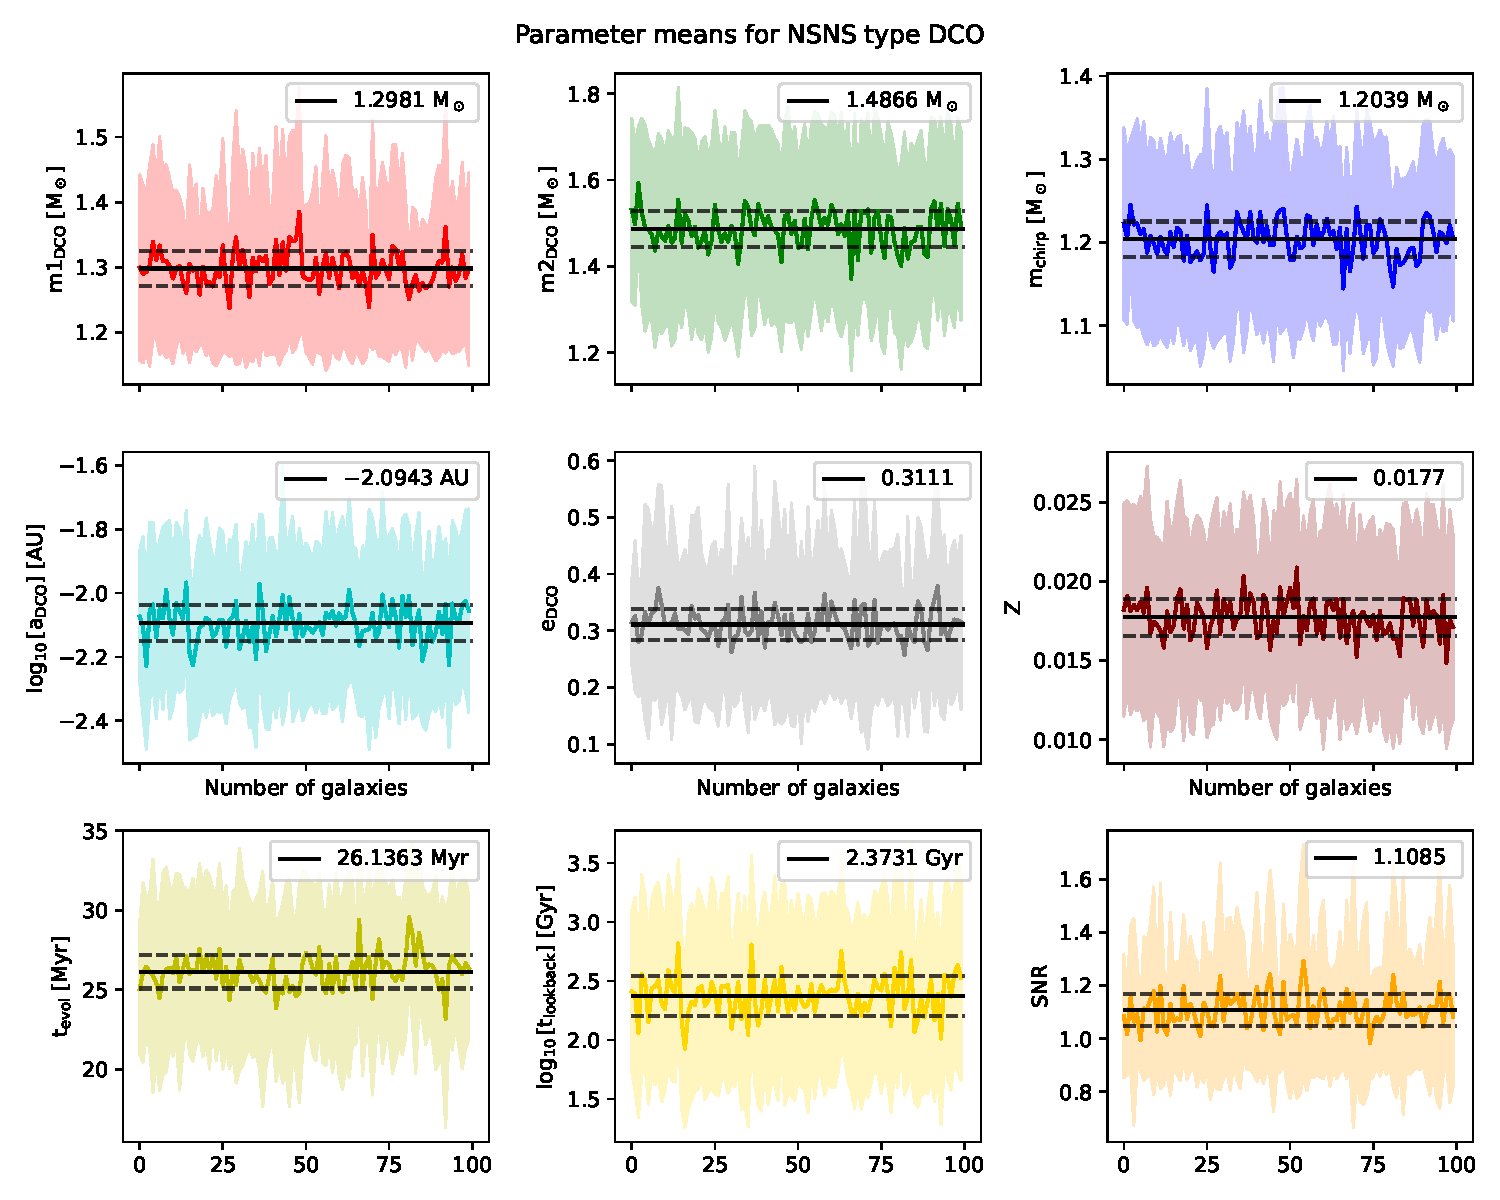
\includegraphics[width=\columnwidth]{analysis_data/main_analysis_folder/NSNS_n_galaxy_mean_plot}
	\caption{Same as figure~\ref{fig:bhbh_n_galaxy_mean_plot}.}
	\label{fig:nsns_n_galaxy_mean_plot}
\end{figure}

\subsection{Neutron Star $-$ Black Hole binary}

\begin{figure}[!h]
	\centering
	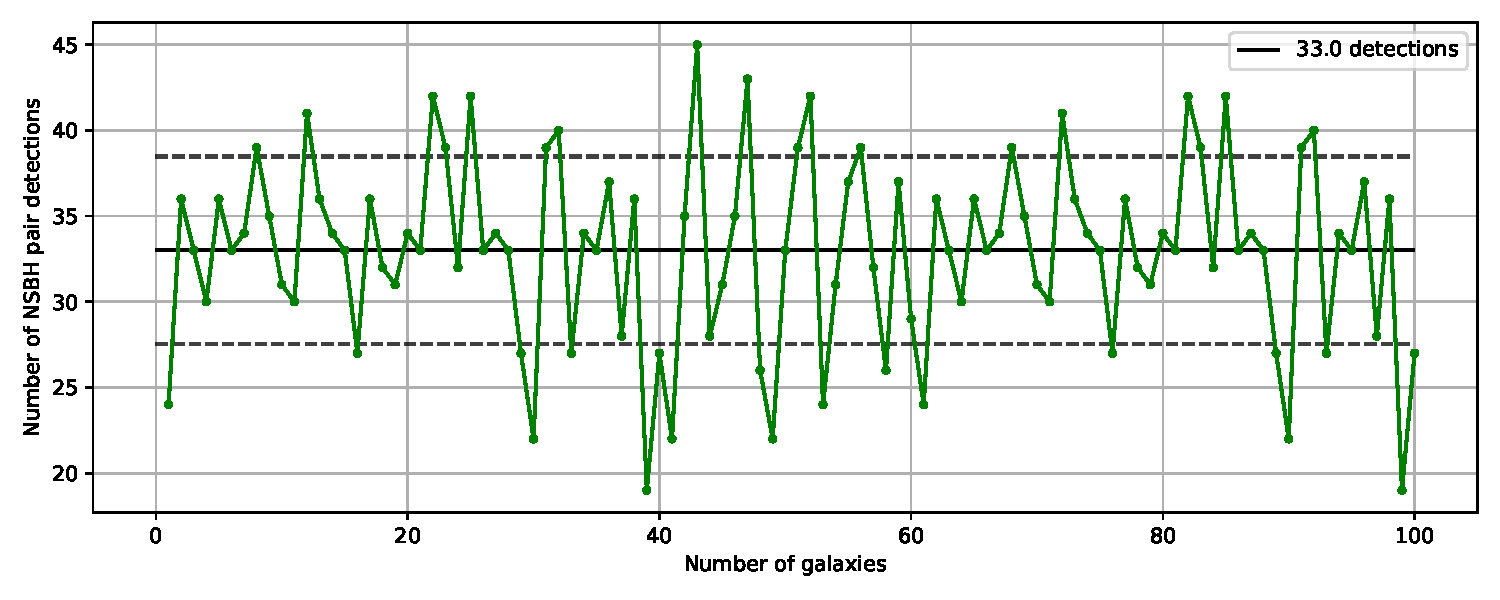
\includegraphics[width=\columnwidth]{analysis_data/main_analysis_folder/NSBH_n_detections}
	\caption{Number of NSBH pair detection per galaxy instance. On average, a total of $\sim$32 pairs per galaxy were detected in this study.}
	\label{fig:nsbhndetections}
\end{figure}	

\begin{figure}[!h]
	\centering
	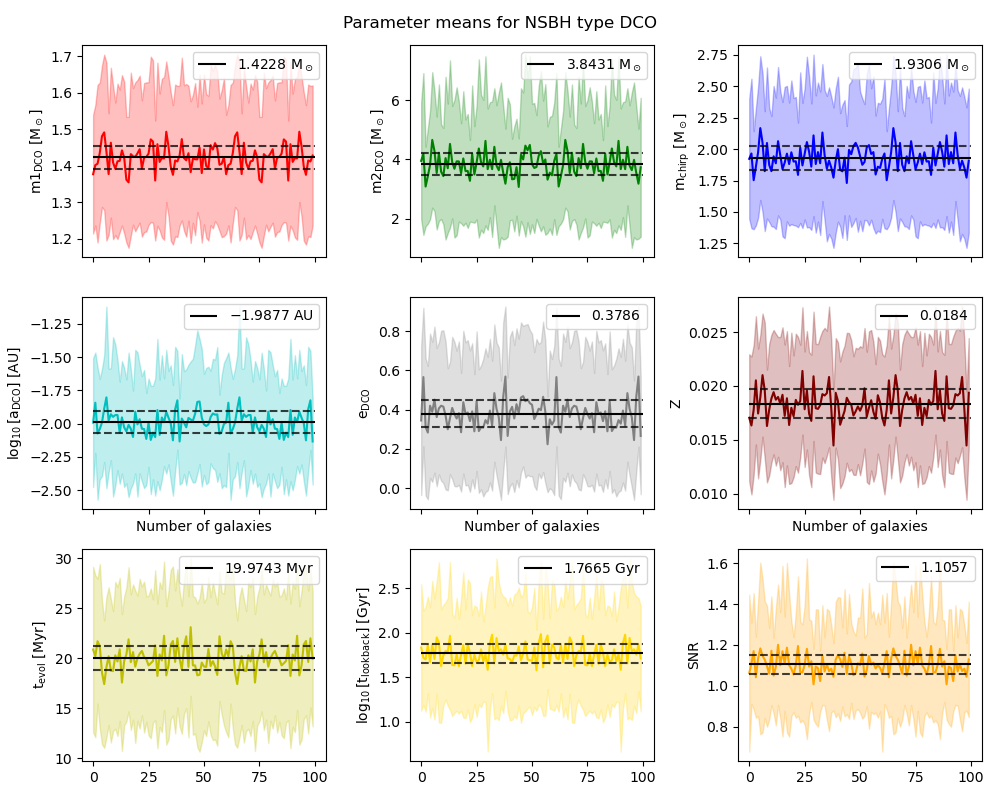
\includegraphics[width=\columnwidth]{analysis_data/main_analysis_folder/NSBH_n_galaxy_mean_plot}
	\caption{Same as figure~\ref{fig:bhbh_n_galaxy_mean_plot}.}
	\label{fig:nsbh_n_galaxy_mean_plot}
\end{figure}

\newpage
\subsection{Black Hole $-$ Neutron Star binary}
\begin{figure}[!h]
	\centering
	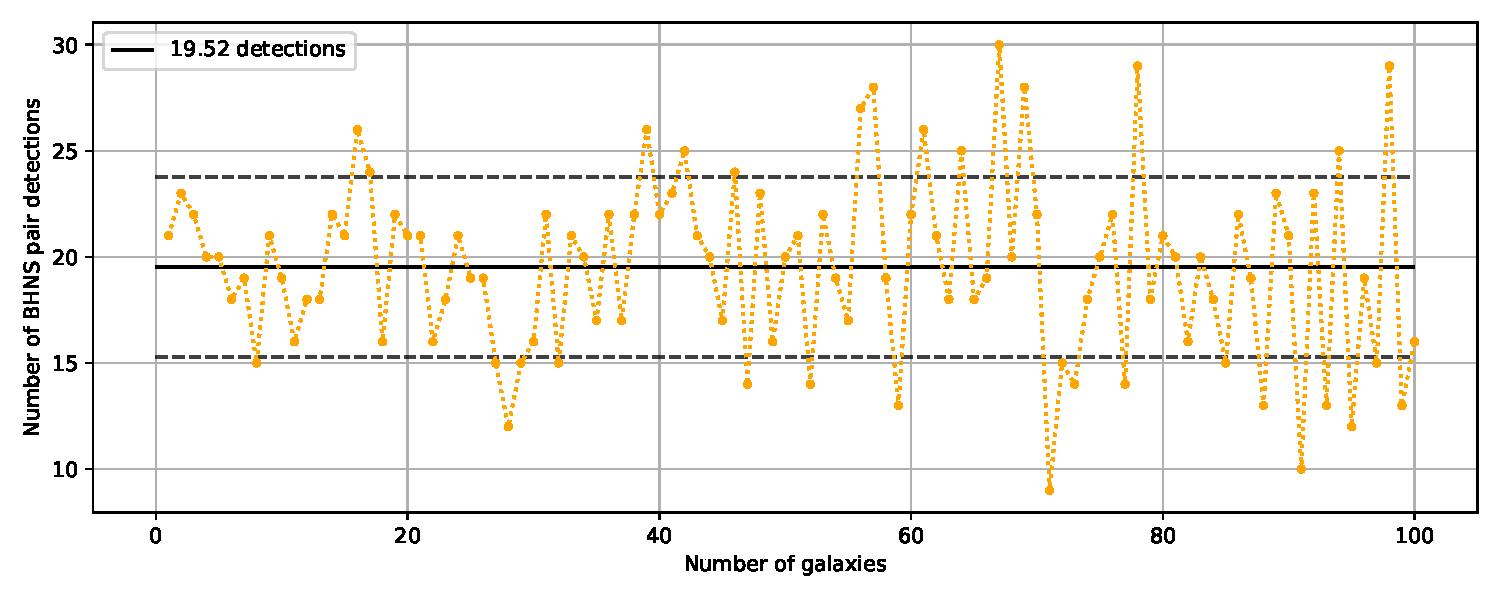
\includegraphics[width=\columnwidth]{analysis_data/main_analysis_folder/BHNS_n_detections}
	\caption{Number of BHNS pair detection per galaxy instance. On average, a total of $\sim$19 pairs per galaxy were detected in this study.}
	\label{fig:bhnsndetections}
\end{figure}	

\begin{figure}[!h]
	\centering
	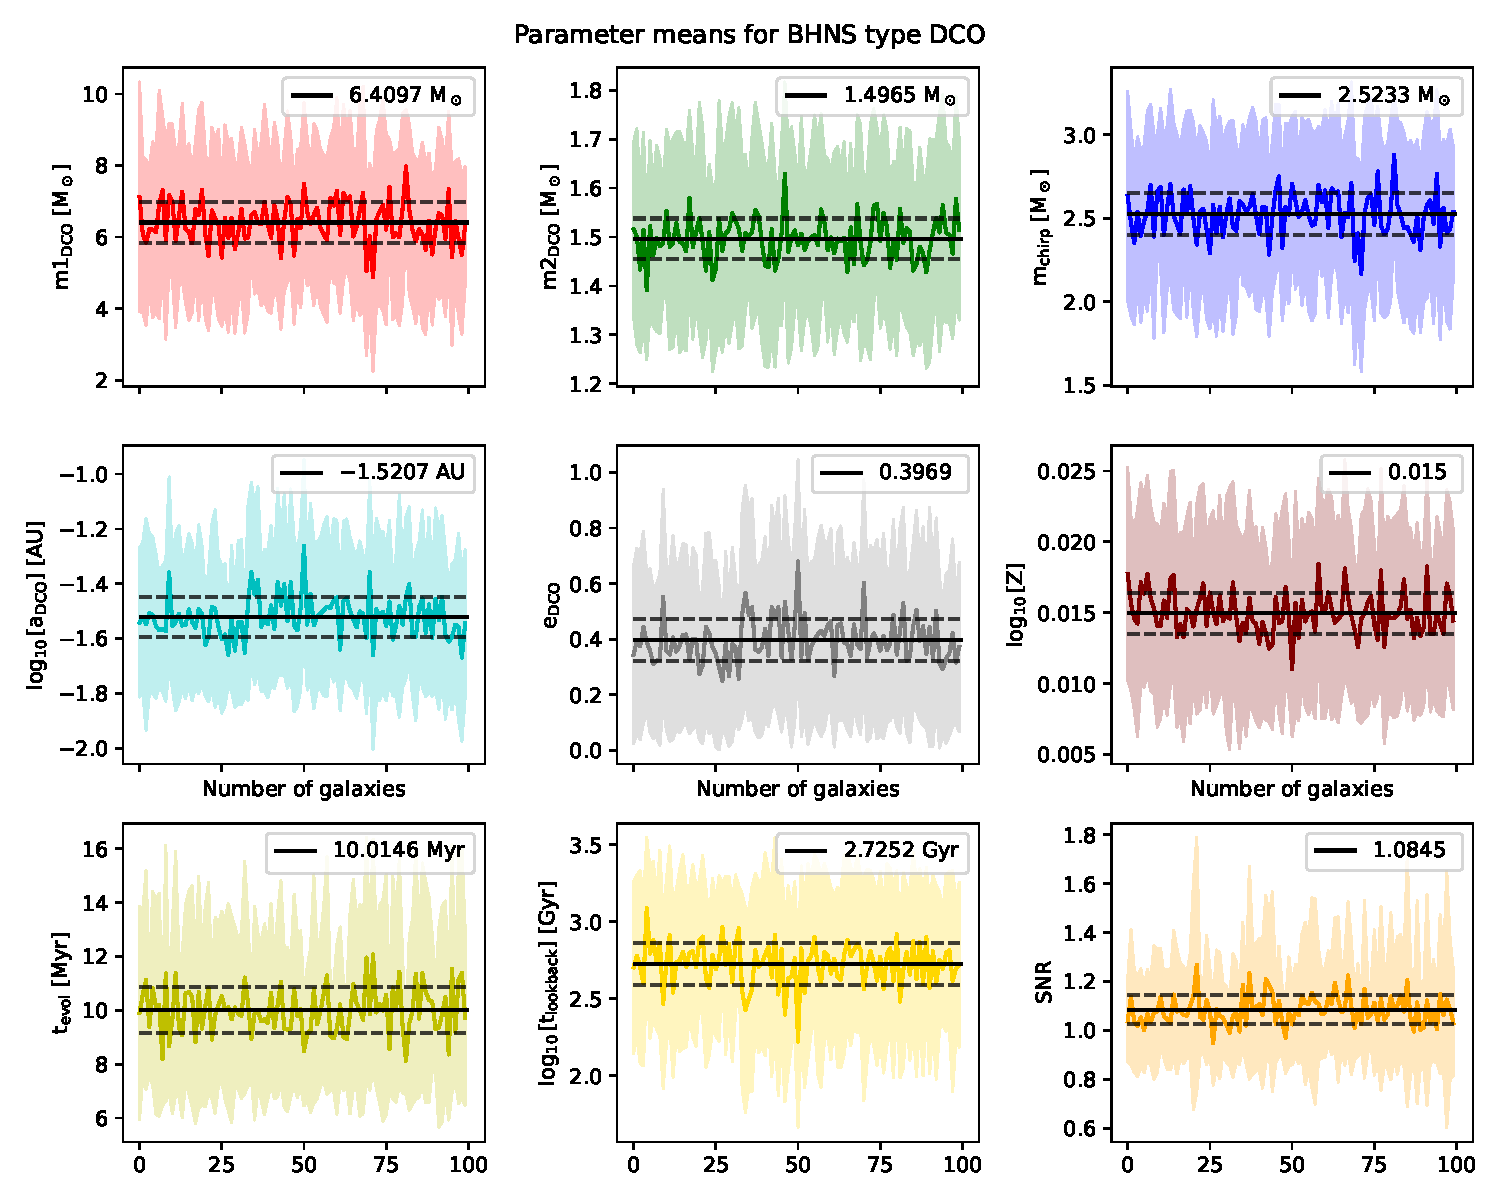
\includegraphics[width=\columnwidth]{analysis_data/main_analysis_folder/BHNS_n_galaxy_mean_plot}
	\caption{Same as figure~\ref{fig:bhbh_n_galaxy_mean_plot}.}
	\label{fig:bhns_n_galaxy_mean_plot}
\end{figure}


\end{document}
